\chapter{Application: Cardiac Mechanics}
\label{chap:5}
%
With the image-based meshing workflow in~\chapref{3} and finite element tools in~\chapref{4} both fully established, the entire image-based modeling and simulation pipeline can now be demonstrated. The application area to be discussed is the mechanical behavior of a beating human heart. Cardiac mechanics is a good testbed for the image-based modeling and simulation workflow described because 1) the application only involves binary image masks, 2) the exact geometry does not grossly affect results since contact modeling is not required, and 3) the use of simulation in this field arguably has the potential to save and improve more lives than any other biomechanics application area.

The primary function of the heart is to pump blood throughout the body, delivering nutrients and removing waste from each organ~\cite{holzapfel_2009}. The cyclic pumping arises from the interaction of its electrical and mechanical function. The heart consists of four chambers: the left ventricle (LV), right ventricle (RV), left atria (LA), and right atria (RA) (See~\figref{anatomy}). The thinner-walled atria act as blood reservoirs for the ventricles, which are responsible for the predominant pumping function. The entire heart is encompassed by a fibrous sac known as the pericardium, which resists rapid increases in cardiac size. Myocardial tissue consists of discrete muscle fiber bundles that exhibit orthotropic material behavior. Refer to Holzapfel \textit{et al.} and Hunter~\cite{schmid} for a more detailed description of the macro and microstructural properties of the heart.

\begin{figure}[htbp!]
\centering
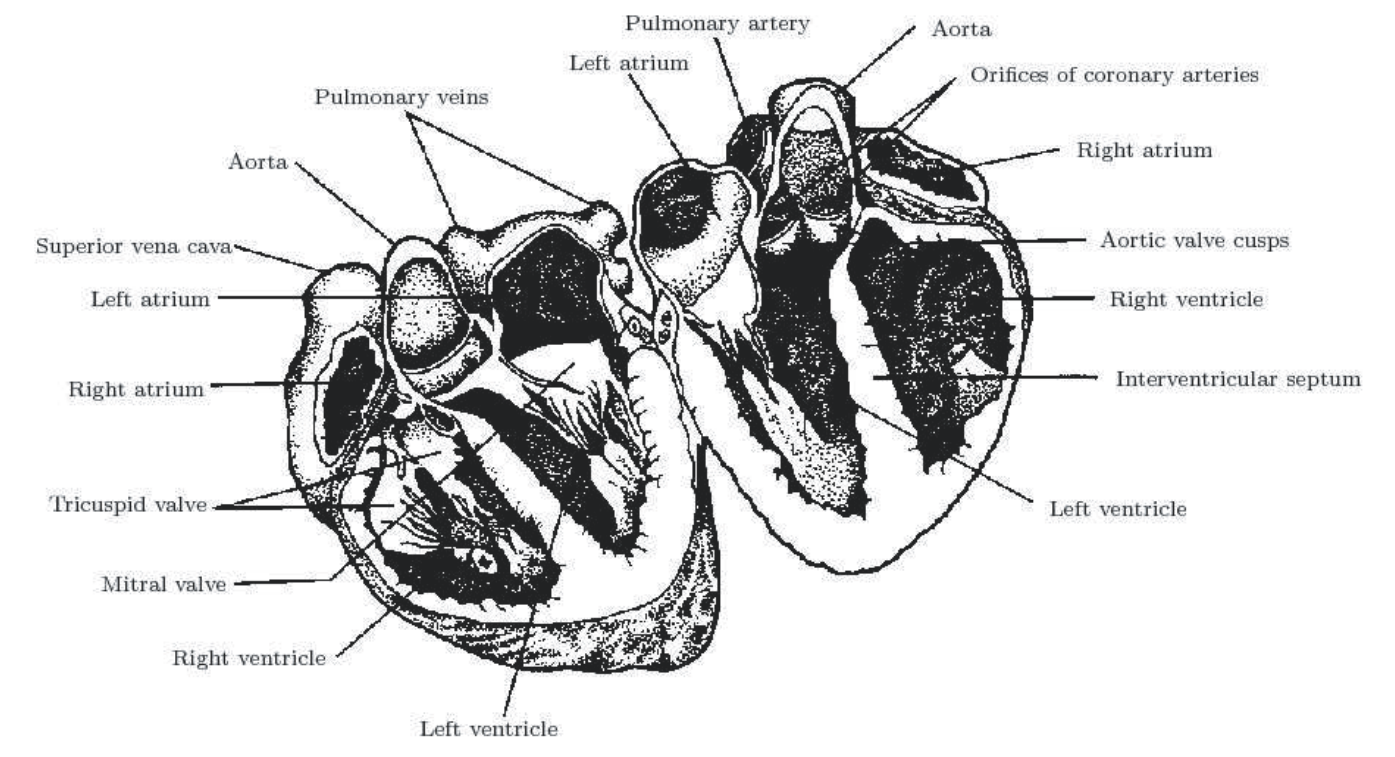
\includegraphics[width=1.0\textwidth]{media/anatomy.png}
\caption{Longitudinal cross-section of the human heart~\cite{katz_2015}}
\label{fig:anatomy}
\end{figure}

Cardiovascular disease is the leading cause of death and disability, accounting for about 40$\%$ of all human mortality~\cite{genet_2015}. Heart failure is one of the most common, costly, and deadly medical conditions, affecting more than 25 million people worldwide~\cite{mann_2015}. Better understanding the nuanced electrical and mechanical behavior of normal and pathological hearts is an important step in improving treatment for heart disease. The complexity of the mechanisms of interest, time and cost savings offered by simulation, and the high sensitivity to various patient-specific parameters make \textit{in silico} modeling an important tool in addressing heart disease.

Cardiac mechanics is one of the most mature fields in computational biomechanics. Several well-known groups have attempted to advance the field from a variety of approaches with respect to the geometry and meshing. \textit{The Living Heart Project}~\cite{baillargeon_2014, genet_2015} has arguably gained the most traction in advancing the understanding of whole-heart cardiac mechanics through simulation, albeit by using linear tetrahedra for a general 50th percentile male heart geometry (i.e., the model was not generated from medical imaging). Augustin \textit{et al.}~\cite{augustin_2016} also used linear tetrahedral finite elements, meshed from smoothed surfaces originating from MRI data. A good deal of informative research still relies on modeling simplified geometries of only the left ventricle~\cite{guccione_2005, sack_2016}, in conjunction even with cubic Hermite finite elements~\cite{mcculloch_2000}. Most modern approaches tend to generate bi-ventricular models (i.e., left and right ventricles) or whole heart models including the atria and potentially even more geometric structures.

Gurev \textit{et al.}~\cite{gurev_2015} performed mechanical simulations on a quadratic hex-dominant mixed element mesh of the human heart ventricles. The work from that group forms the basis for most of the cardiac mechanics explorations to be discussed in this chapter. The review article by Trayanova \textit{et al.}~\cite{trayanova_2011} provides an excellent summary of the components to ventricular electromechanical modeling utilized by the papers mentioned above.

These essential components to computational cardiac mechanics are described in this chapter for an implementation using conventional finite elements, namely: mesh generation, material model characterization, muscle fiber orientation, boundary conditions, the solver. Simulation results are also presented. Finally, the details of implementing the same mechanics into the polyhedral code \textit{Celeris} are discussed, along with preliminary verification results.

%%%%%%%%%%%%%%%%%%%%%%%%%%%%%%%%%%%%%%%%%%%%%%%
%%%%%%%%%%%%%%%%%%%%%%%%%%%%%%%%%%%%%%%%%%%%%%%
\section{Methods}
\label{Methods}

Description of Cardioid here

%%%%%%%%%%%%%%%%%%%%%%%%%%%%%%%%%%%%%%%%%%%%%%%
%%%%%%%%%%%%%%%%%%%%%%%%%%%%%%%%%%%%%%%%%%%%%%%
\subsection{Mesh Generation}
\label{Mesh Generation}

Again quadratic tetrahedral elements are chosen as over linear elements to avoid volumetric locking and impracticably fine meshes to yield accurate results.

Oomph
Describe generation of segs and meshes: \\
threshold \\
level set \\
connected components \\
fill holes \\
dilate-erode \\
manual fine-tuning \\

~\figref{tet2}

%%%%%%%%%%%%%%%%%%%%%%%%%%%%%%%%%%%%%%%%%%%%%%%
%%%%%%%%%%%%%%%%%%%%%%%%%%%%%%%%%%%%%%%%%%%%%%%
\subsection{Material Model}
\label{Material Model}

\subsubsection{Passive Stress}
\label{Passive Stress}

\subsubsection{Active Stress}
\label{Active Stress}

%%%%%%%%%%%%%%%%%%%%%%%%%%%%%%%%%%%%%%%%%%%%%%%
%%%%%%%%%%%%%%%%%%%%%%%%%%%%%%%%%%%%%%%%%%%%%%%
\subsection{Fiber Generation}
\label{Fiber Generation}

\begin{figure}[ht]
\centering
\subfigure[]{%
		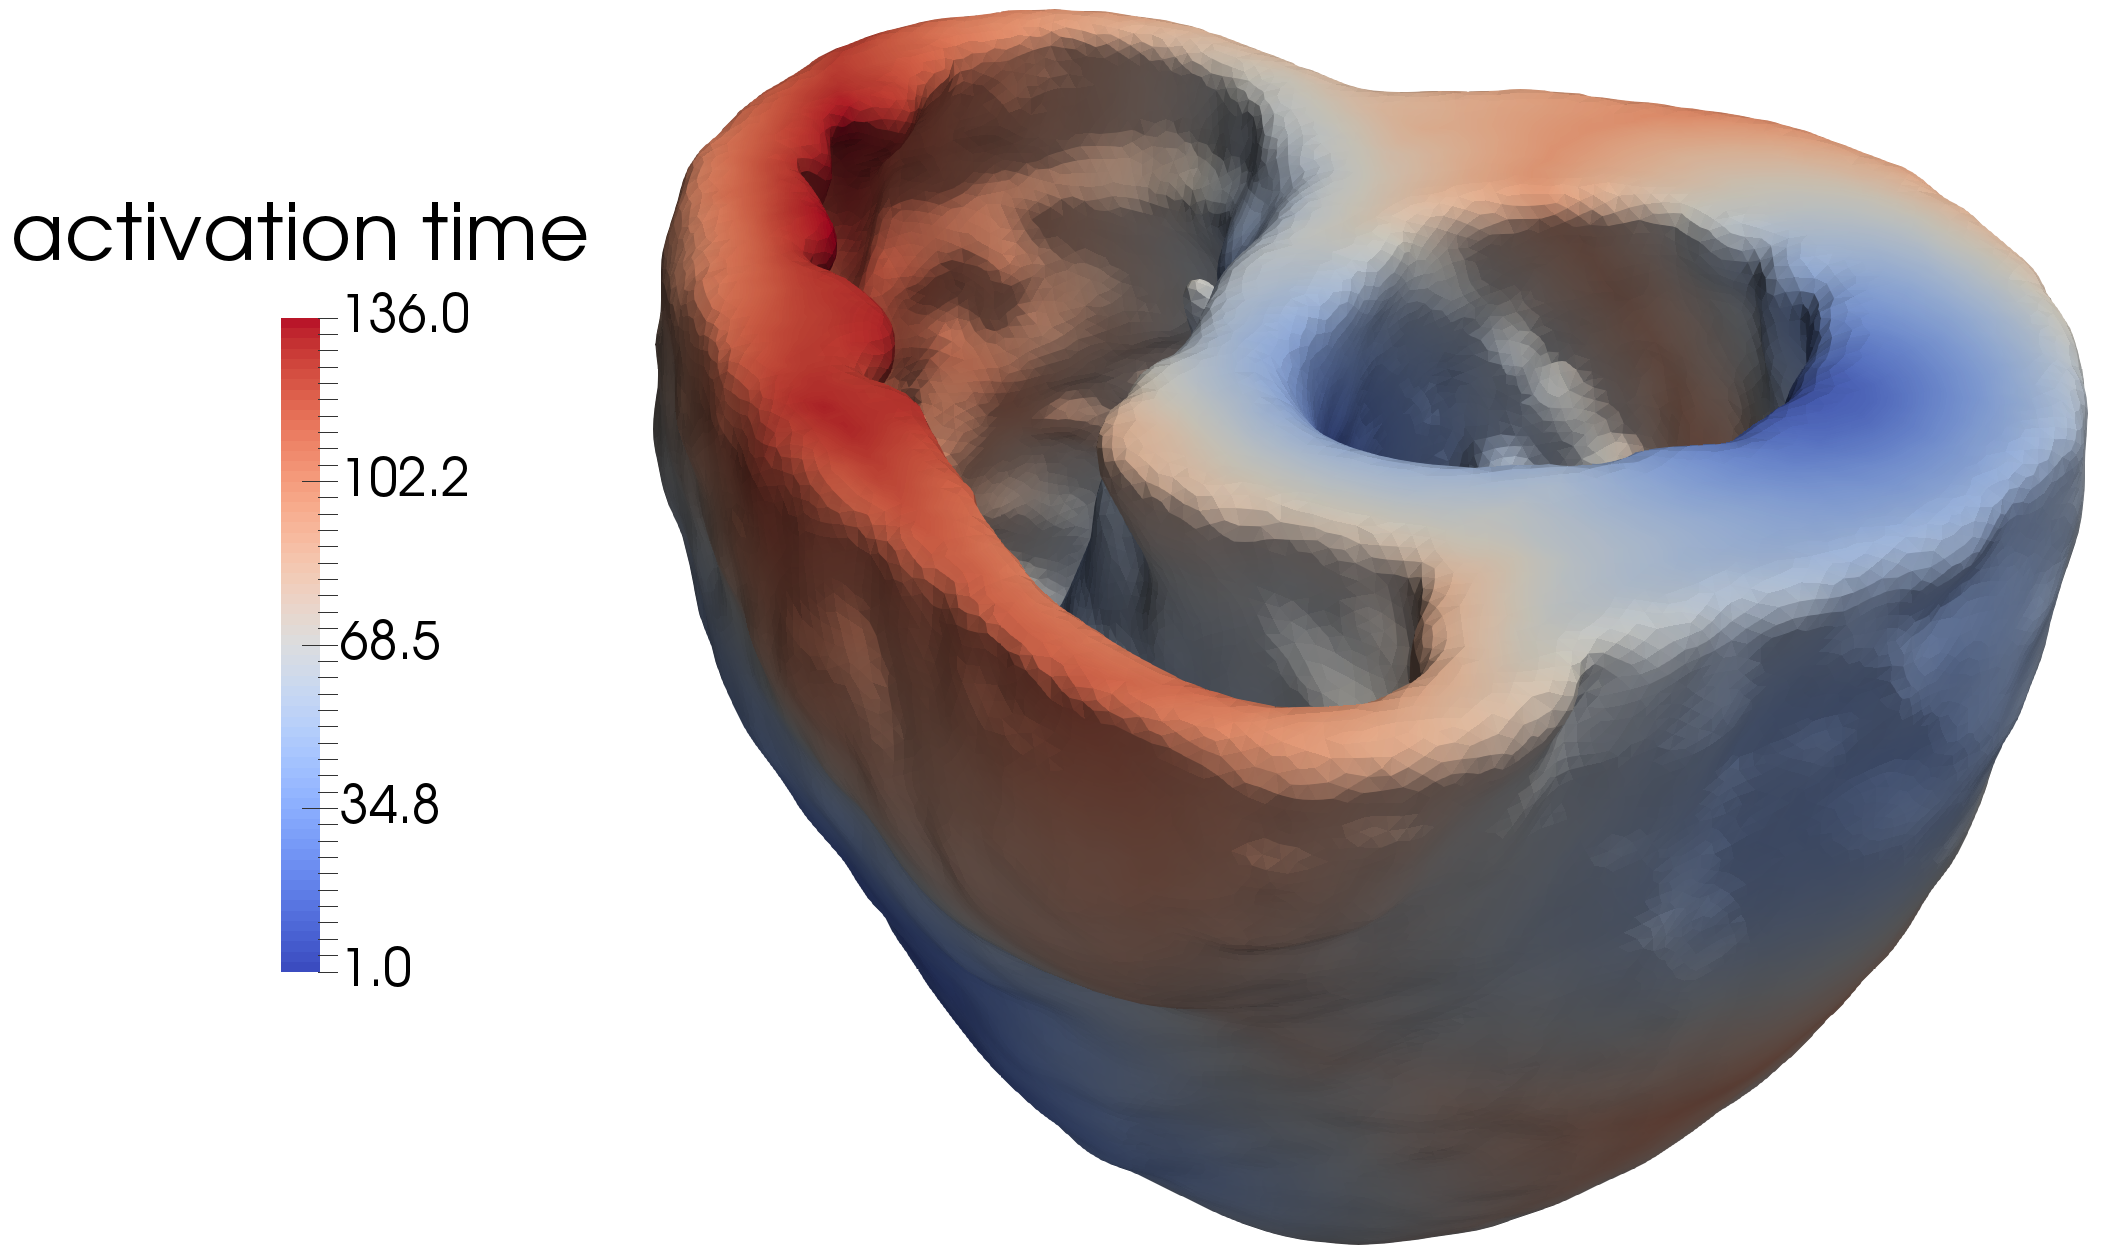
\includegraphics[scale=0.081]{media/4-cardioid/2-activationtime.png}
\label{fig:supp1}}
\subfigure[]{%
		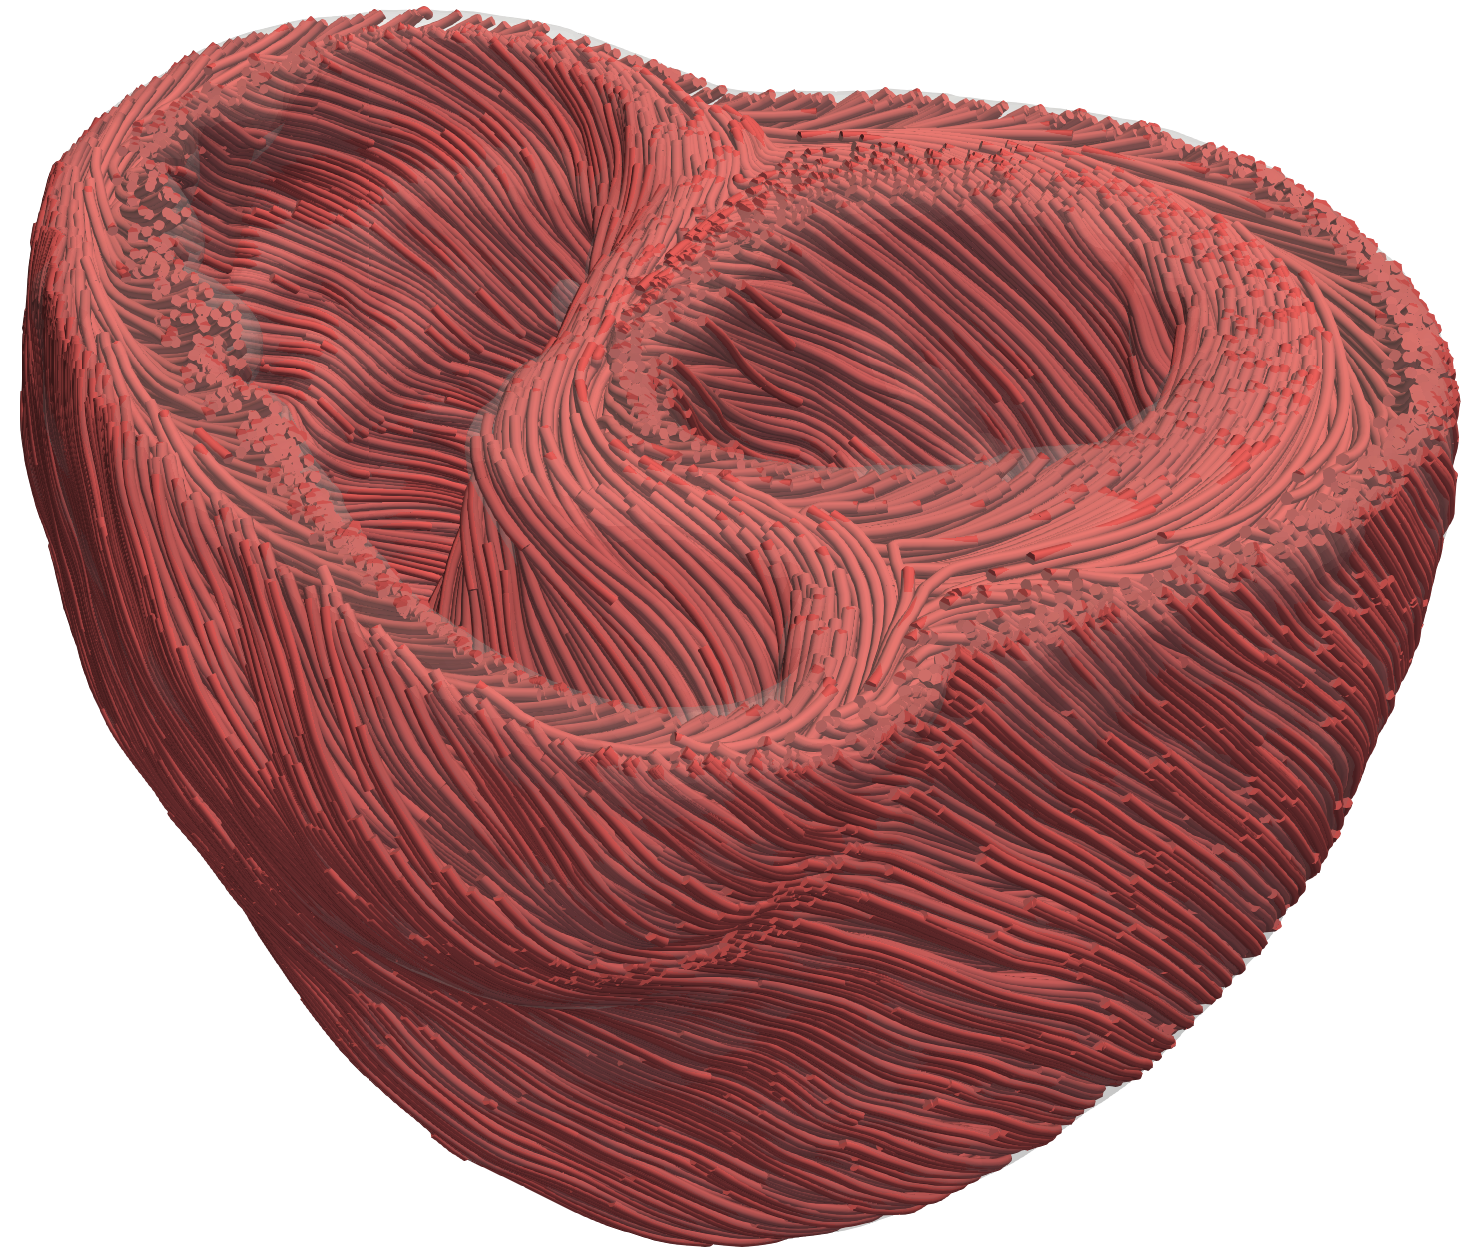
\includegraphics[scale=0.081]{media/4-cardioid/3-fibers.png}
\label{fig:supp2}}
\subfigure[]{%
		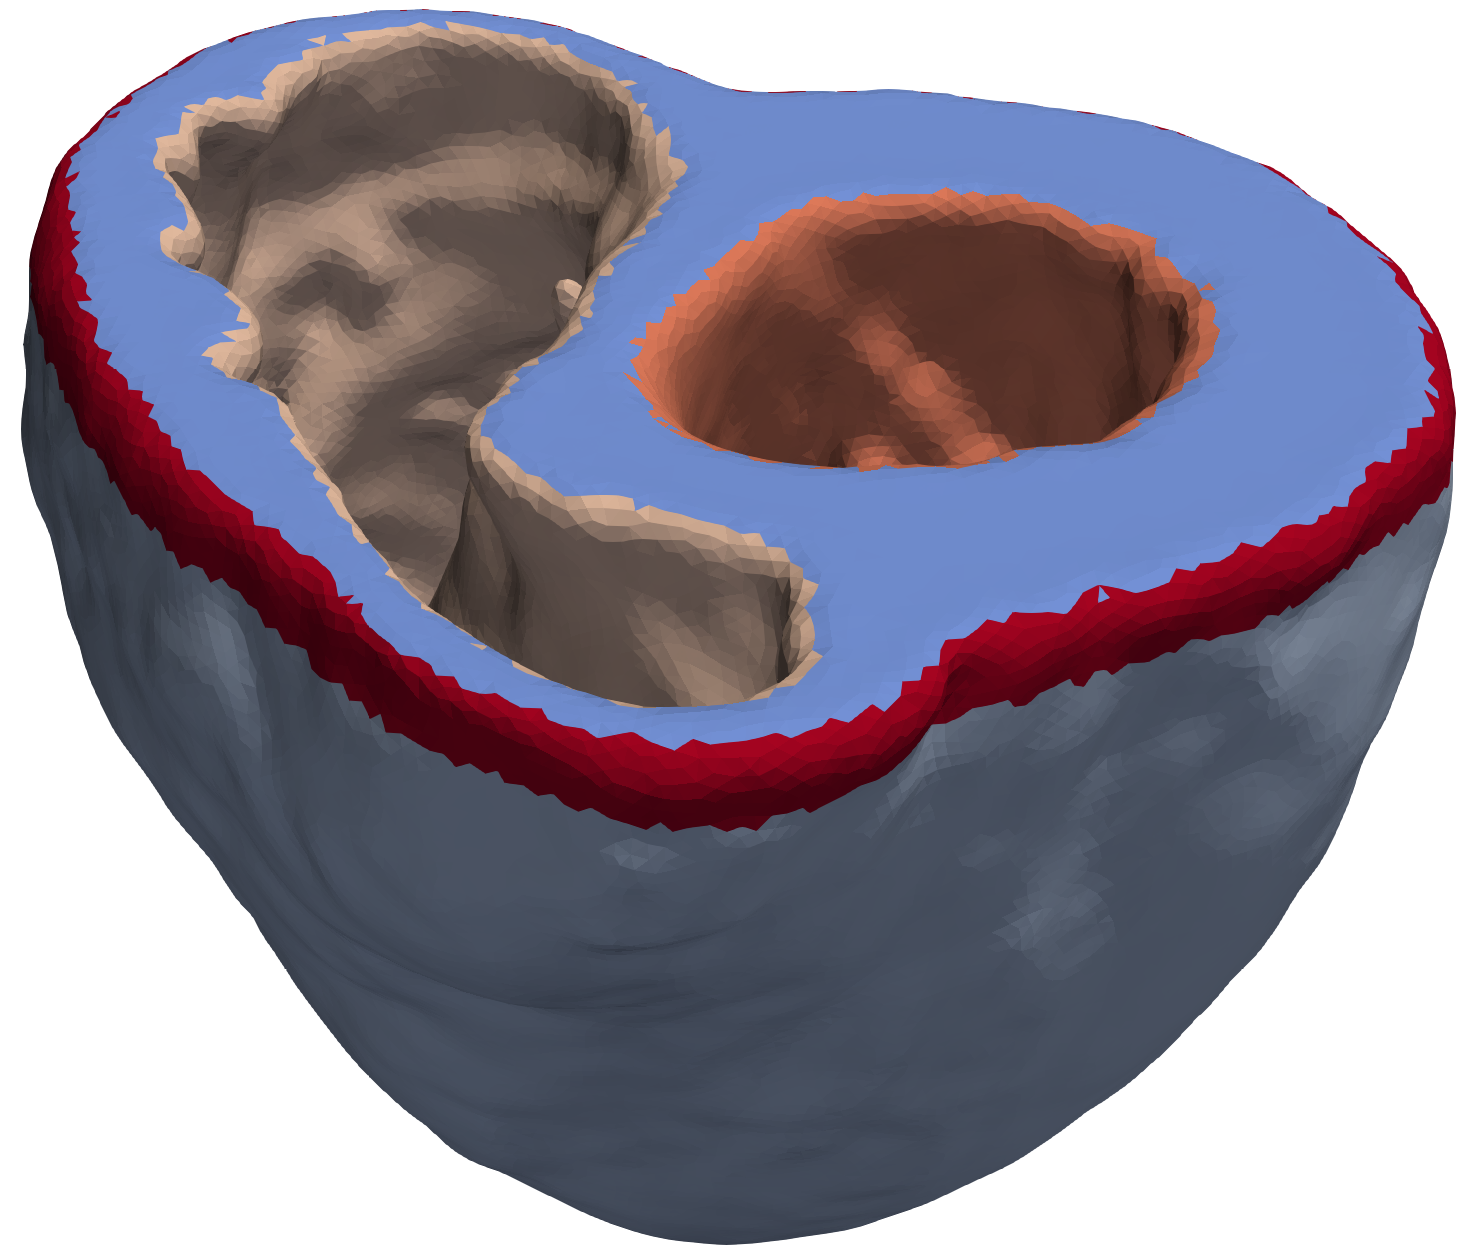
\includegraphics[scale=0.081]{media/4-cardioid/4-tagged.png}
\label{fig:supp3}}
%
\caption{Mechanics modeling considerations: (a) muscle fiber orientations, (b) electrical activation times, and c) surface tagging and prescription of corresponding boundary conditions.}
\label{fig:supp}
\end{figure}

%%%%%%%%%%%%%%%%%%%%%%%%%%%%%%%%%%%%%%%%%%%%%%%
%%%%%%%%%%%%%%%%%%%%%%%%%%%%%%%%%%%%%%%%%%%%%%%
\subsection{Boundary Conditions}
\label{Boundary Conditions}

%%%%%%%%%%%%%%%%%%%%%%%%%%%%%%%%%%%%%%%%%%%%%%%
%%%%%%%%%%%%%%%%%%%%%%%%%%%%%%%%%%%%%%%%%%%%%%%
\subsection{Solver}
\label{Solver}

%%%%%%%%%%%%%%%%%%%%%%%%%%%%%%%%%%%%%%%%%%%%%%%
%%%%%%%%%%%%%%%%%%%%%%%%%%%%%%%%%%%%%%%%%%%%%%%
\section{Results}
\label{Results}


\begin{figure}[ht]
\centering
\subfigure[]{%
		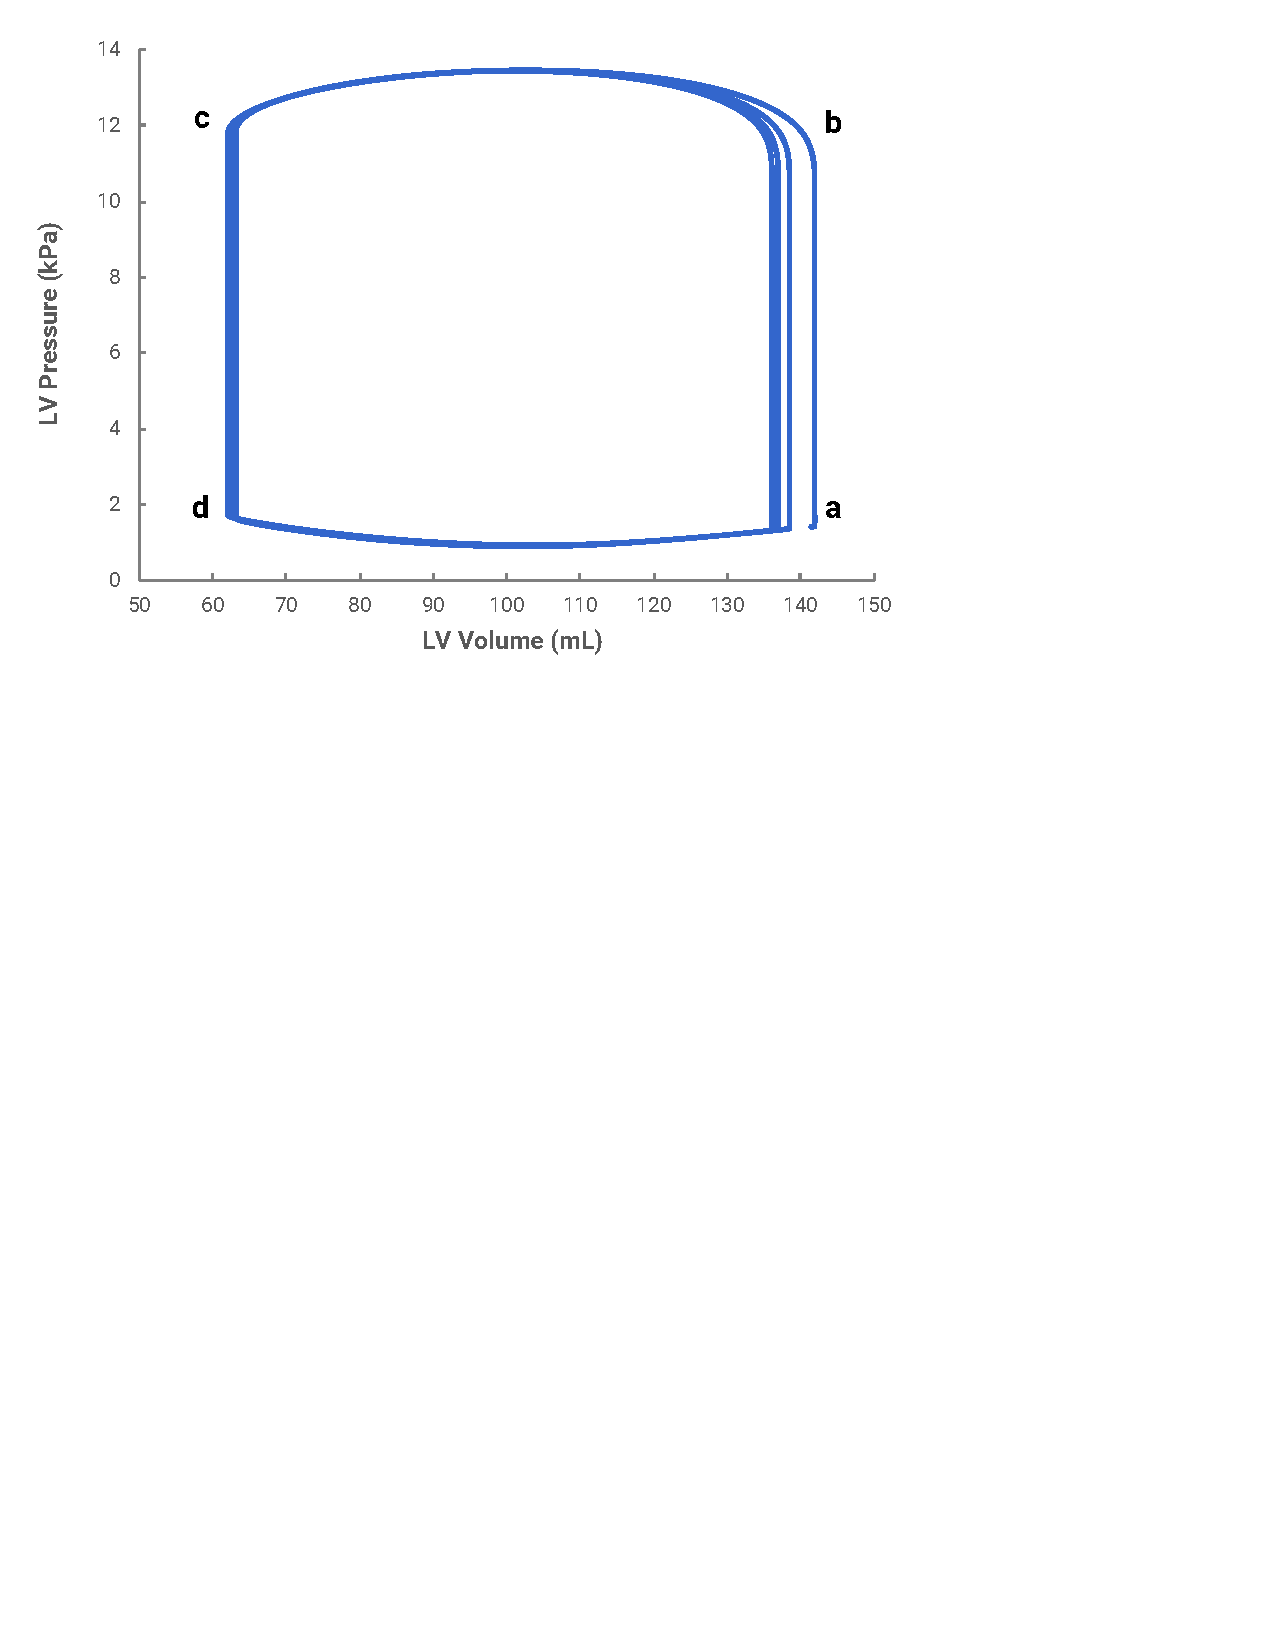
\includegraphics[scale=0.5]{media/4-cardioid/5-pv/pressure_volume-1.pdf}
\label{fig:pv1}}		
\subfigure[]{%
		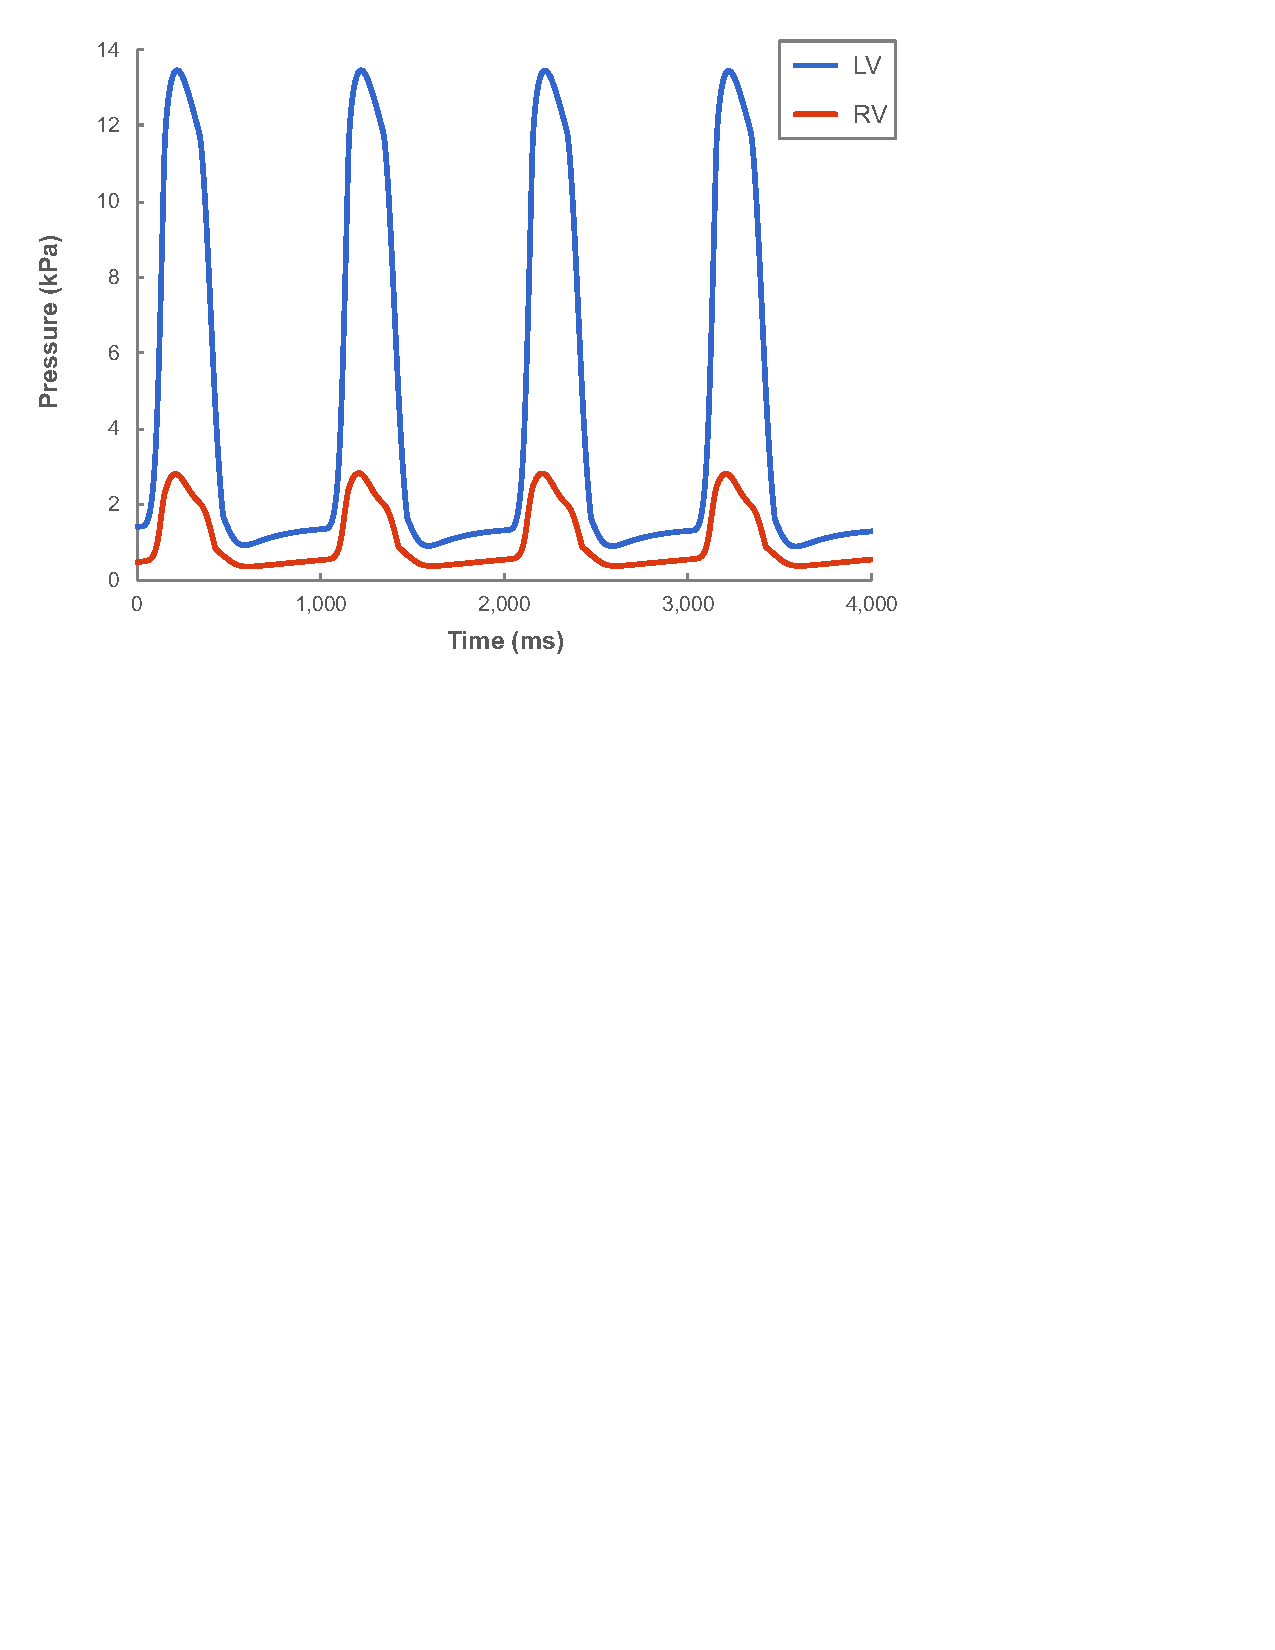
\includegraphics[scale=0.5]{media/4-cardioid/5-pv/pressure_volume-2.pdf}
\label{fig:pv2}}		
%
\caption{Results from Cardioid simulation: (a) P-V loop of left ventricle, (b) pressure time history in left and right ventricles.}
\label{fig:pv}
\end{figure}

\begin{figure}[ht!]
\centering
\subfigure[]{%
		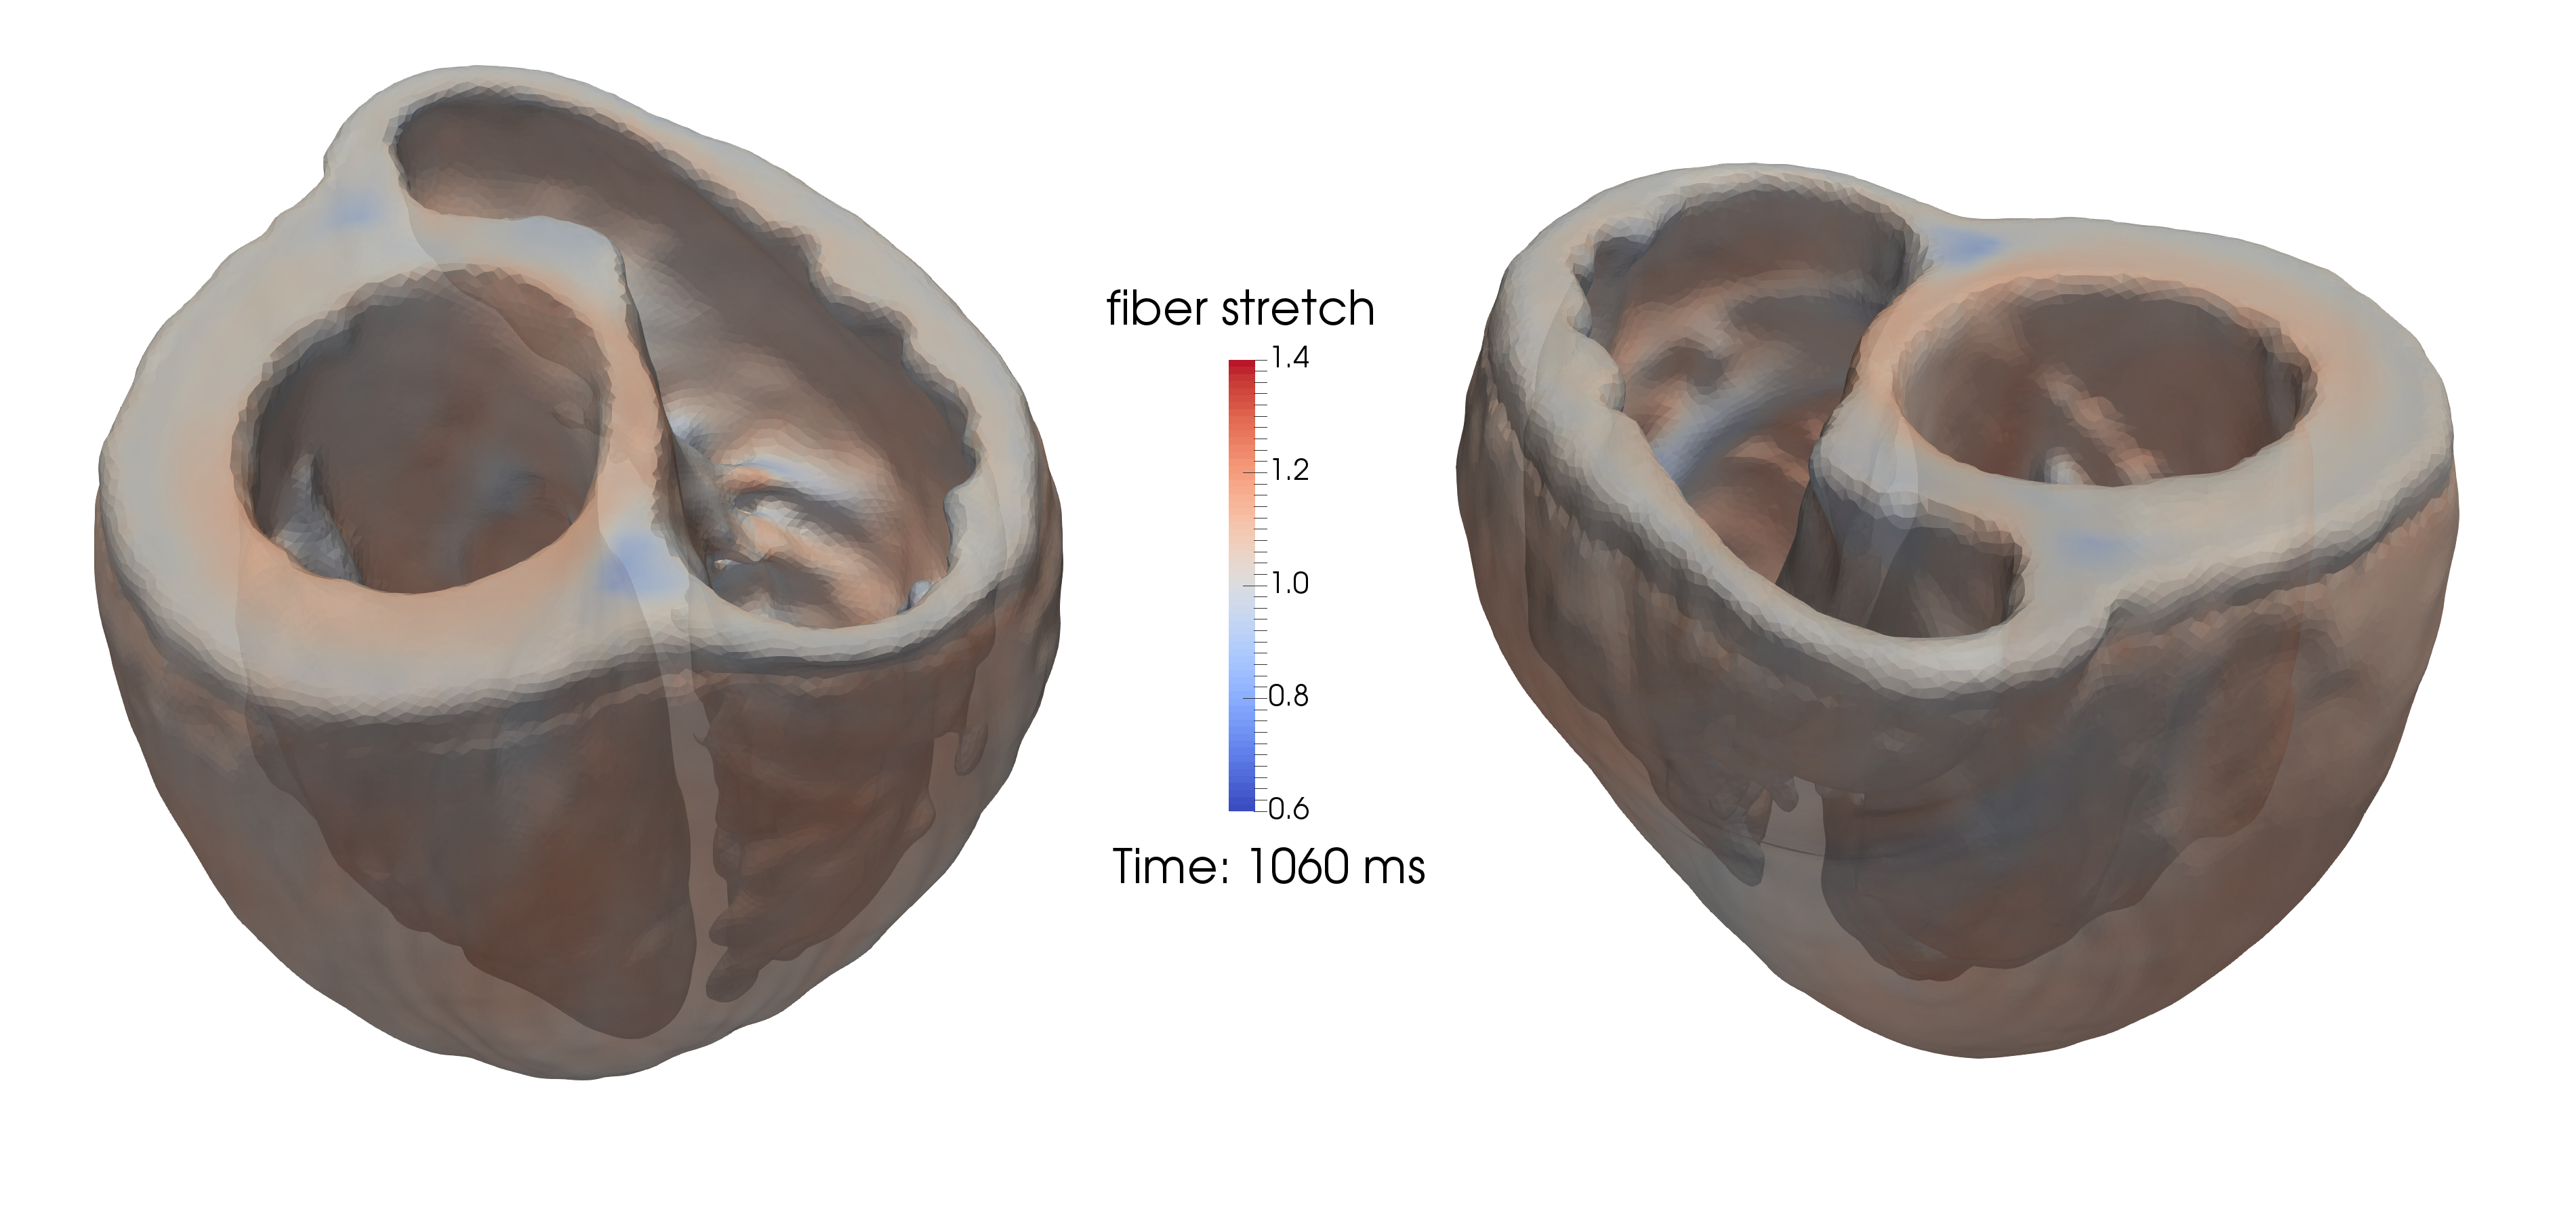
\includegraphics[scale=0.057]{media/4-cardioid/6-vid/a.png}
\label{fig:snaps1}}		
\subfigure[]{%
		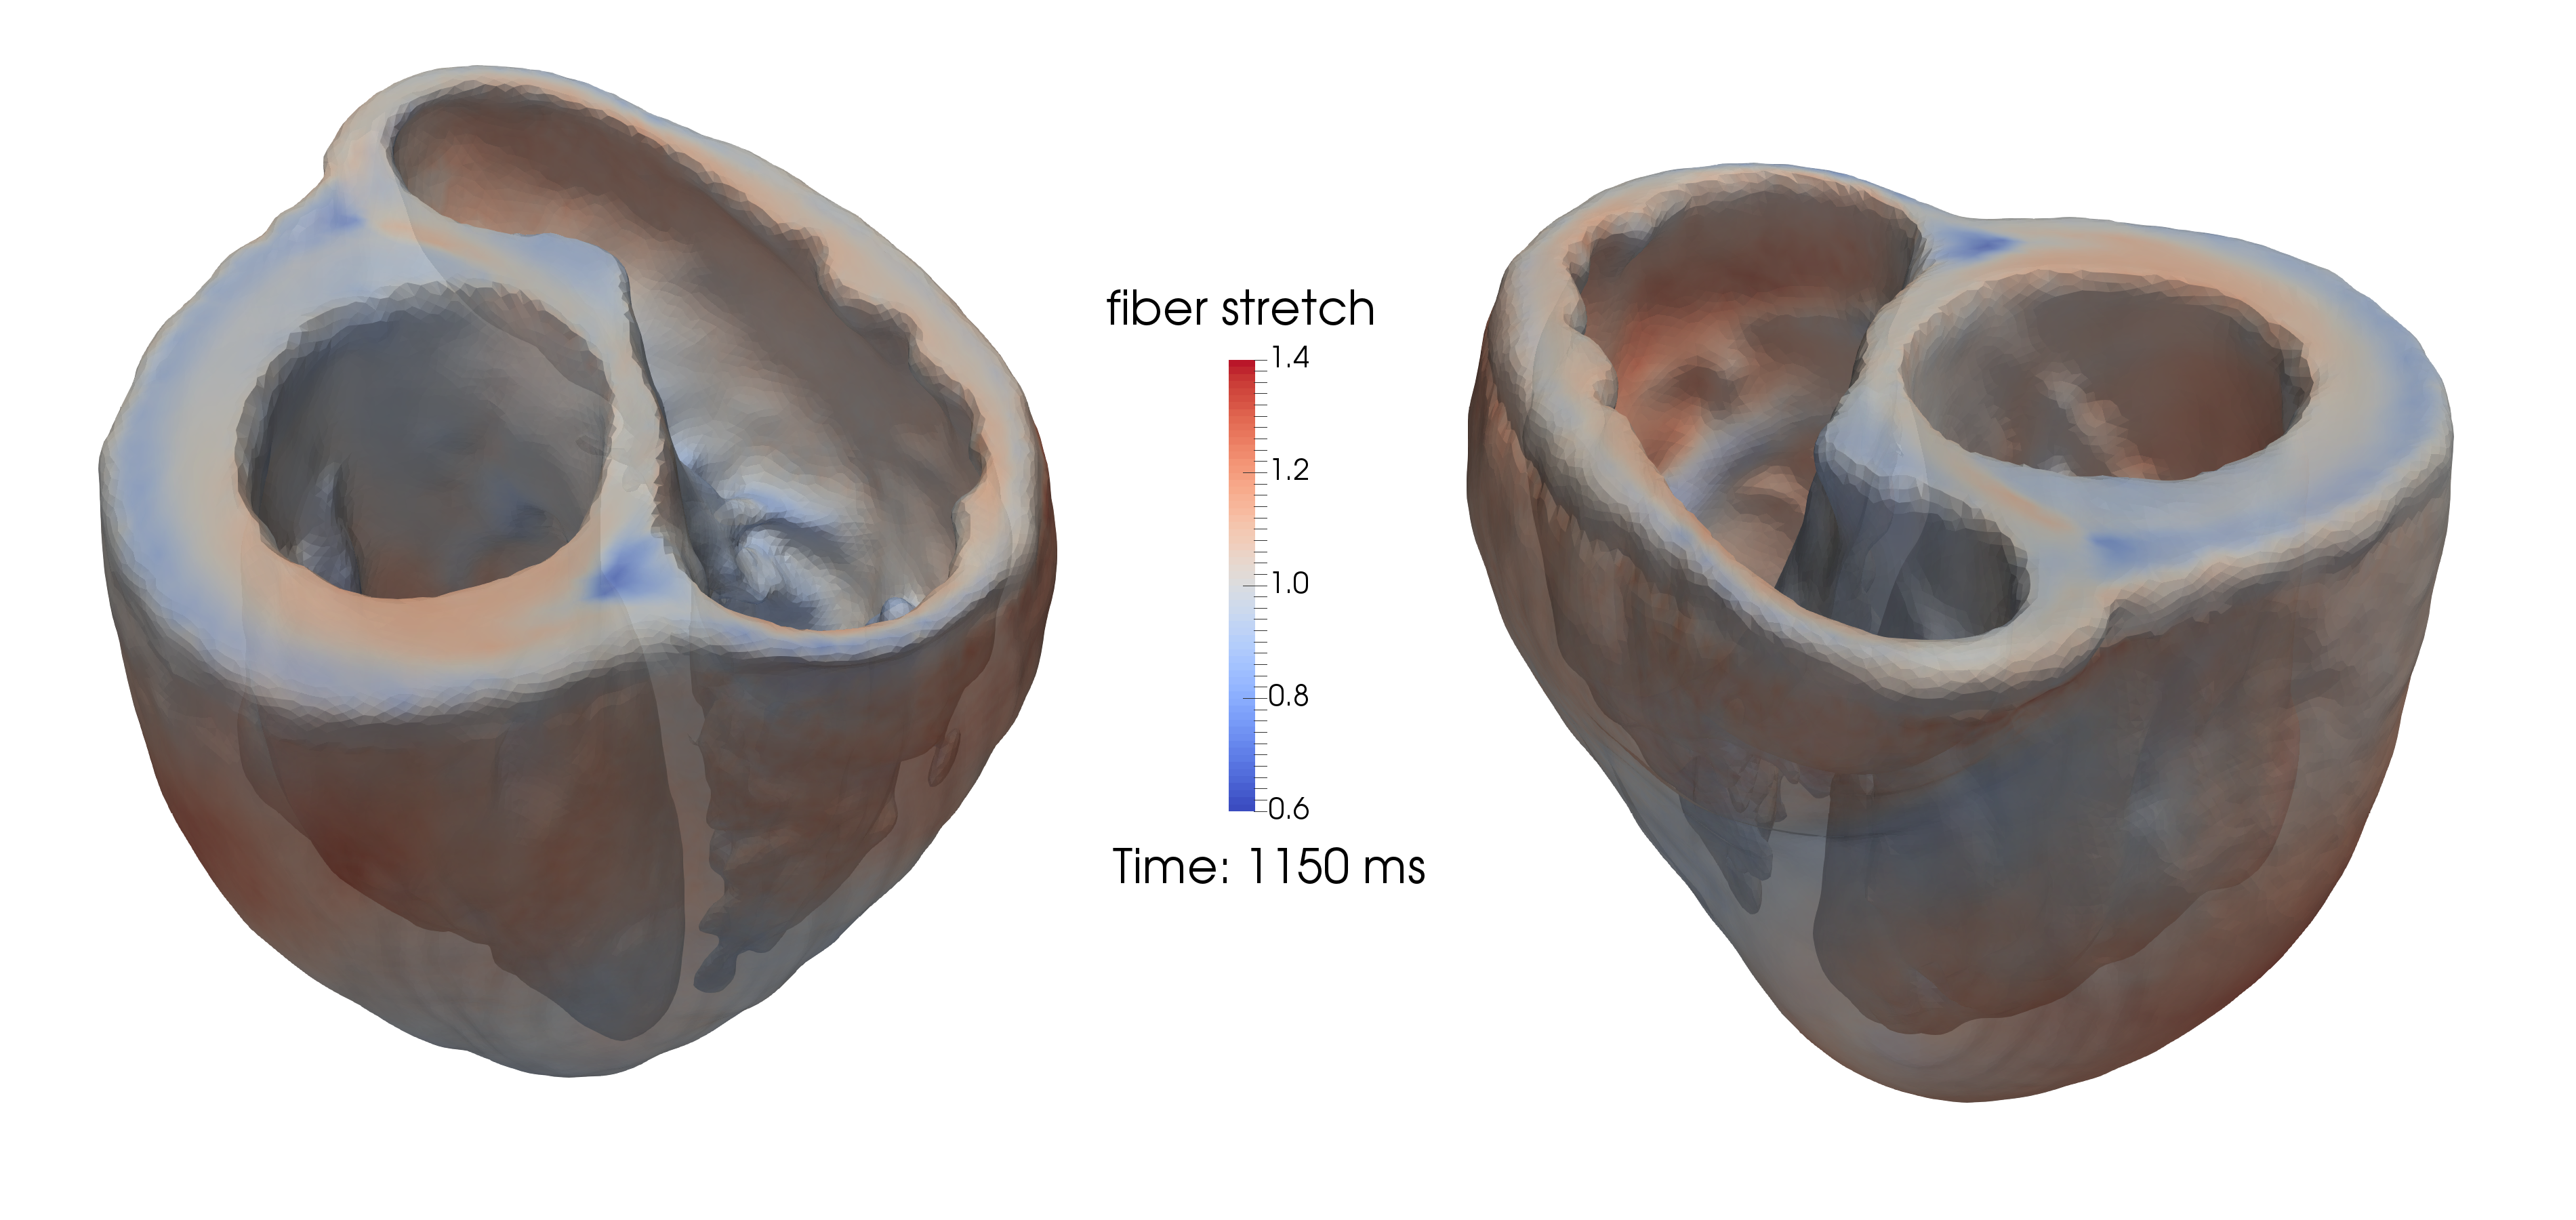
\includegraphics[scale=0.057]{media/4-cardioid/6-vid/b.png}
\label{fig:snaps2}}		
\subfigure[]{%
		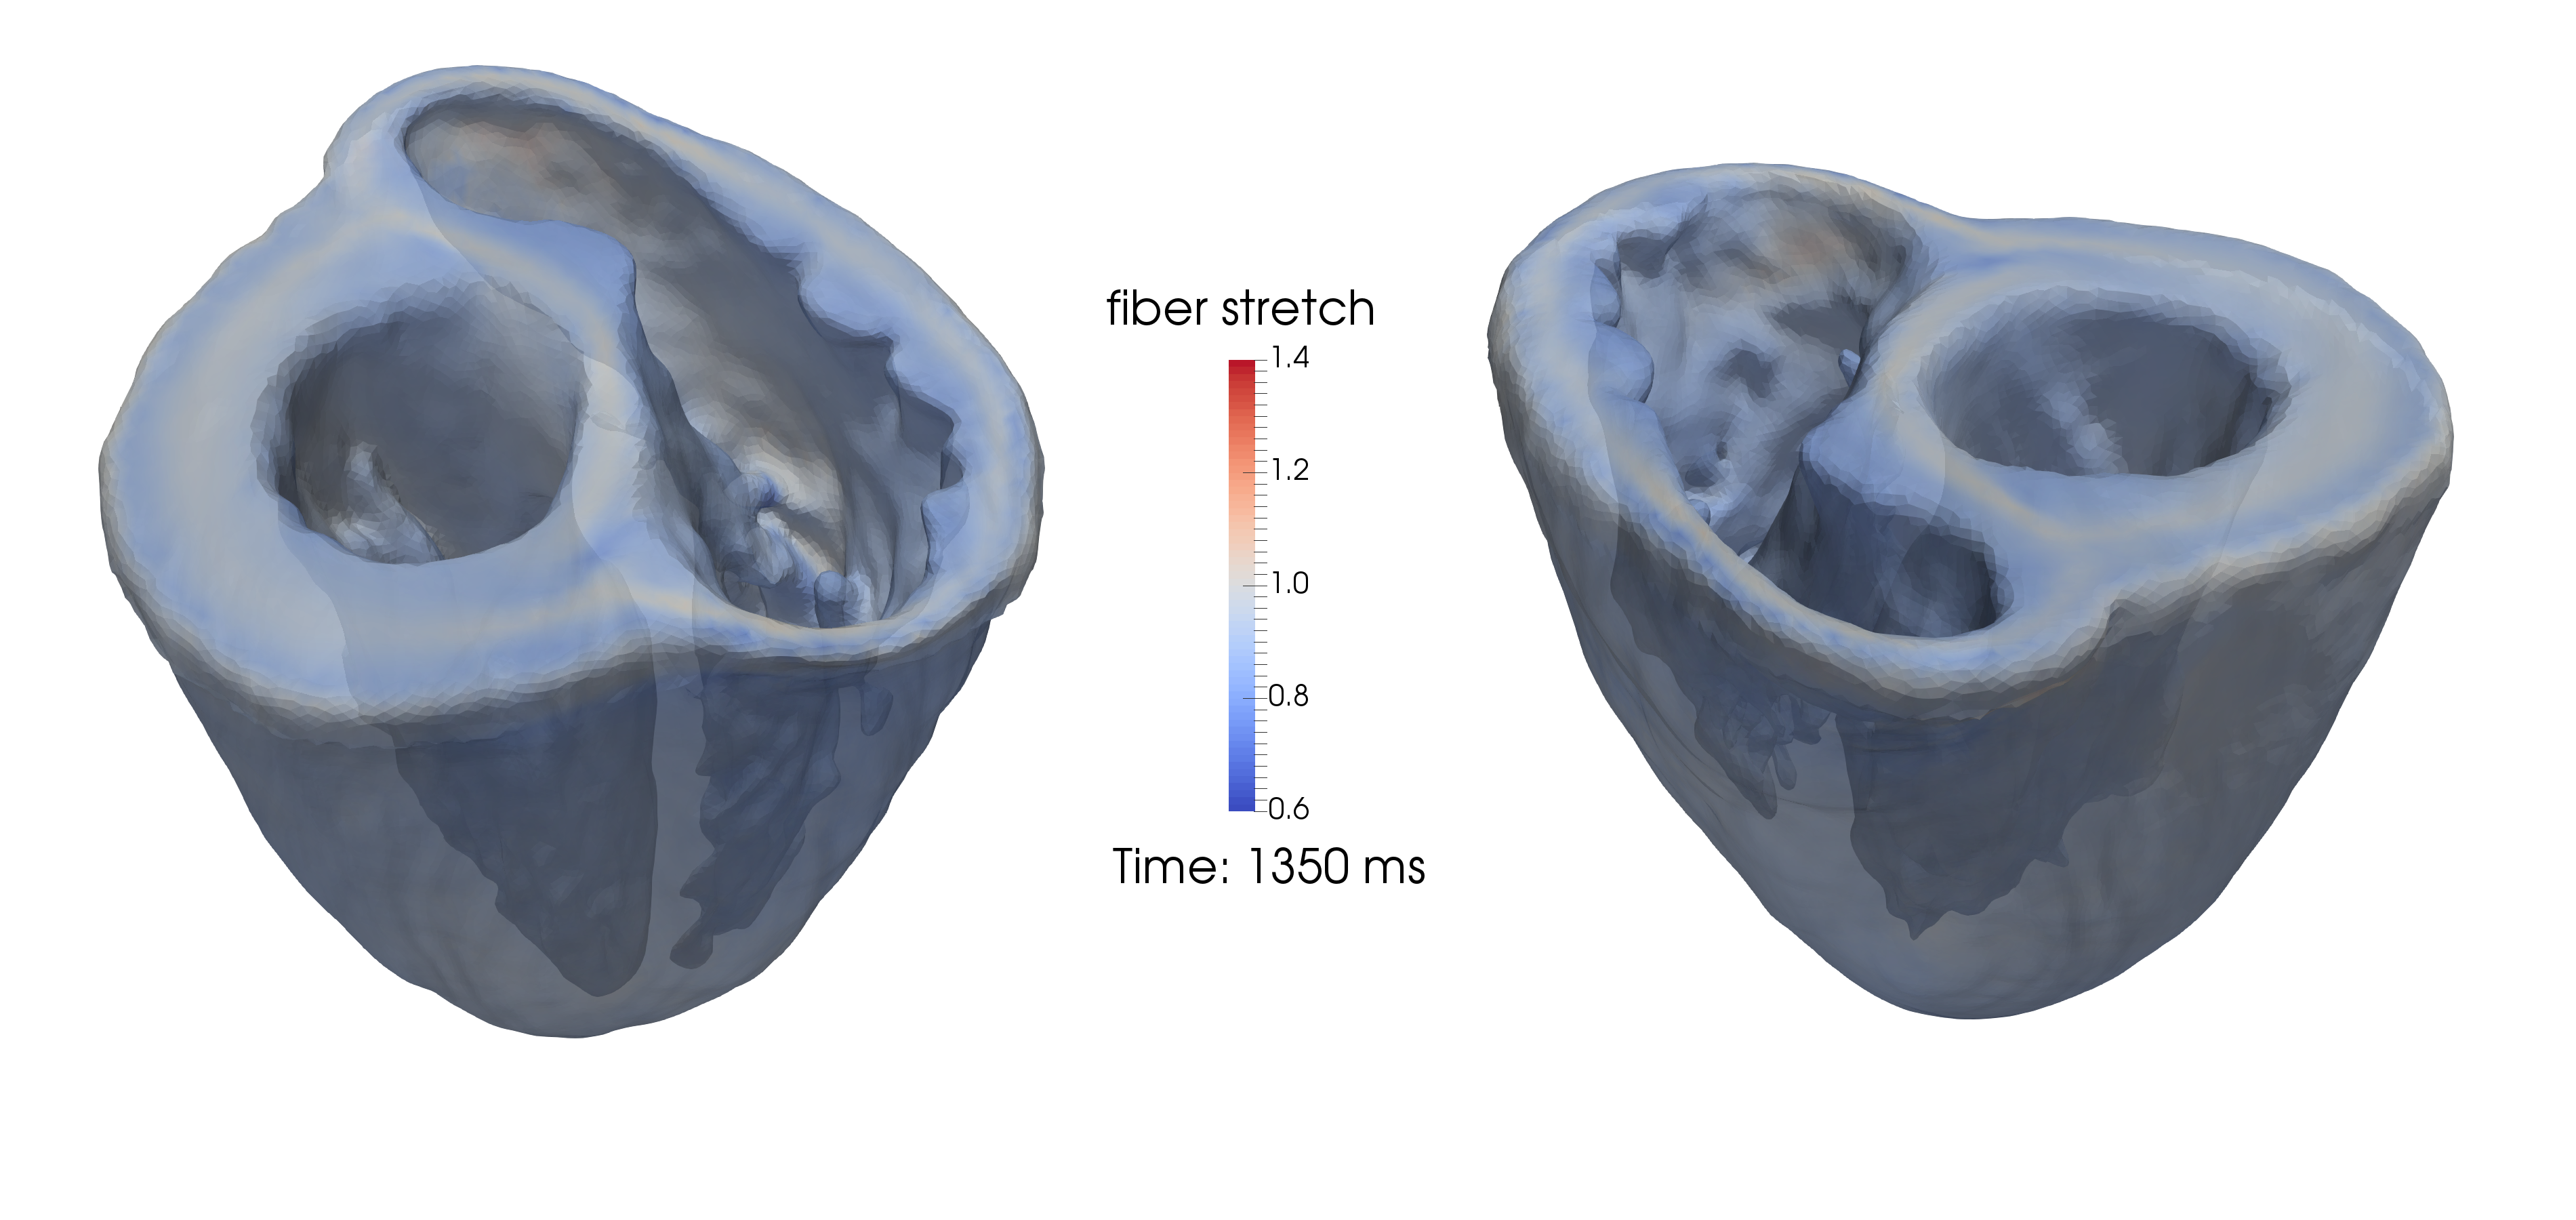
\includegraphics[scale=0.057]{media/4-cardioid/6-vid/c.png}
\label{fig:snapsf3}}		
\subfigure[]{%
		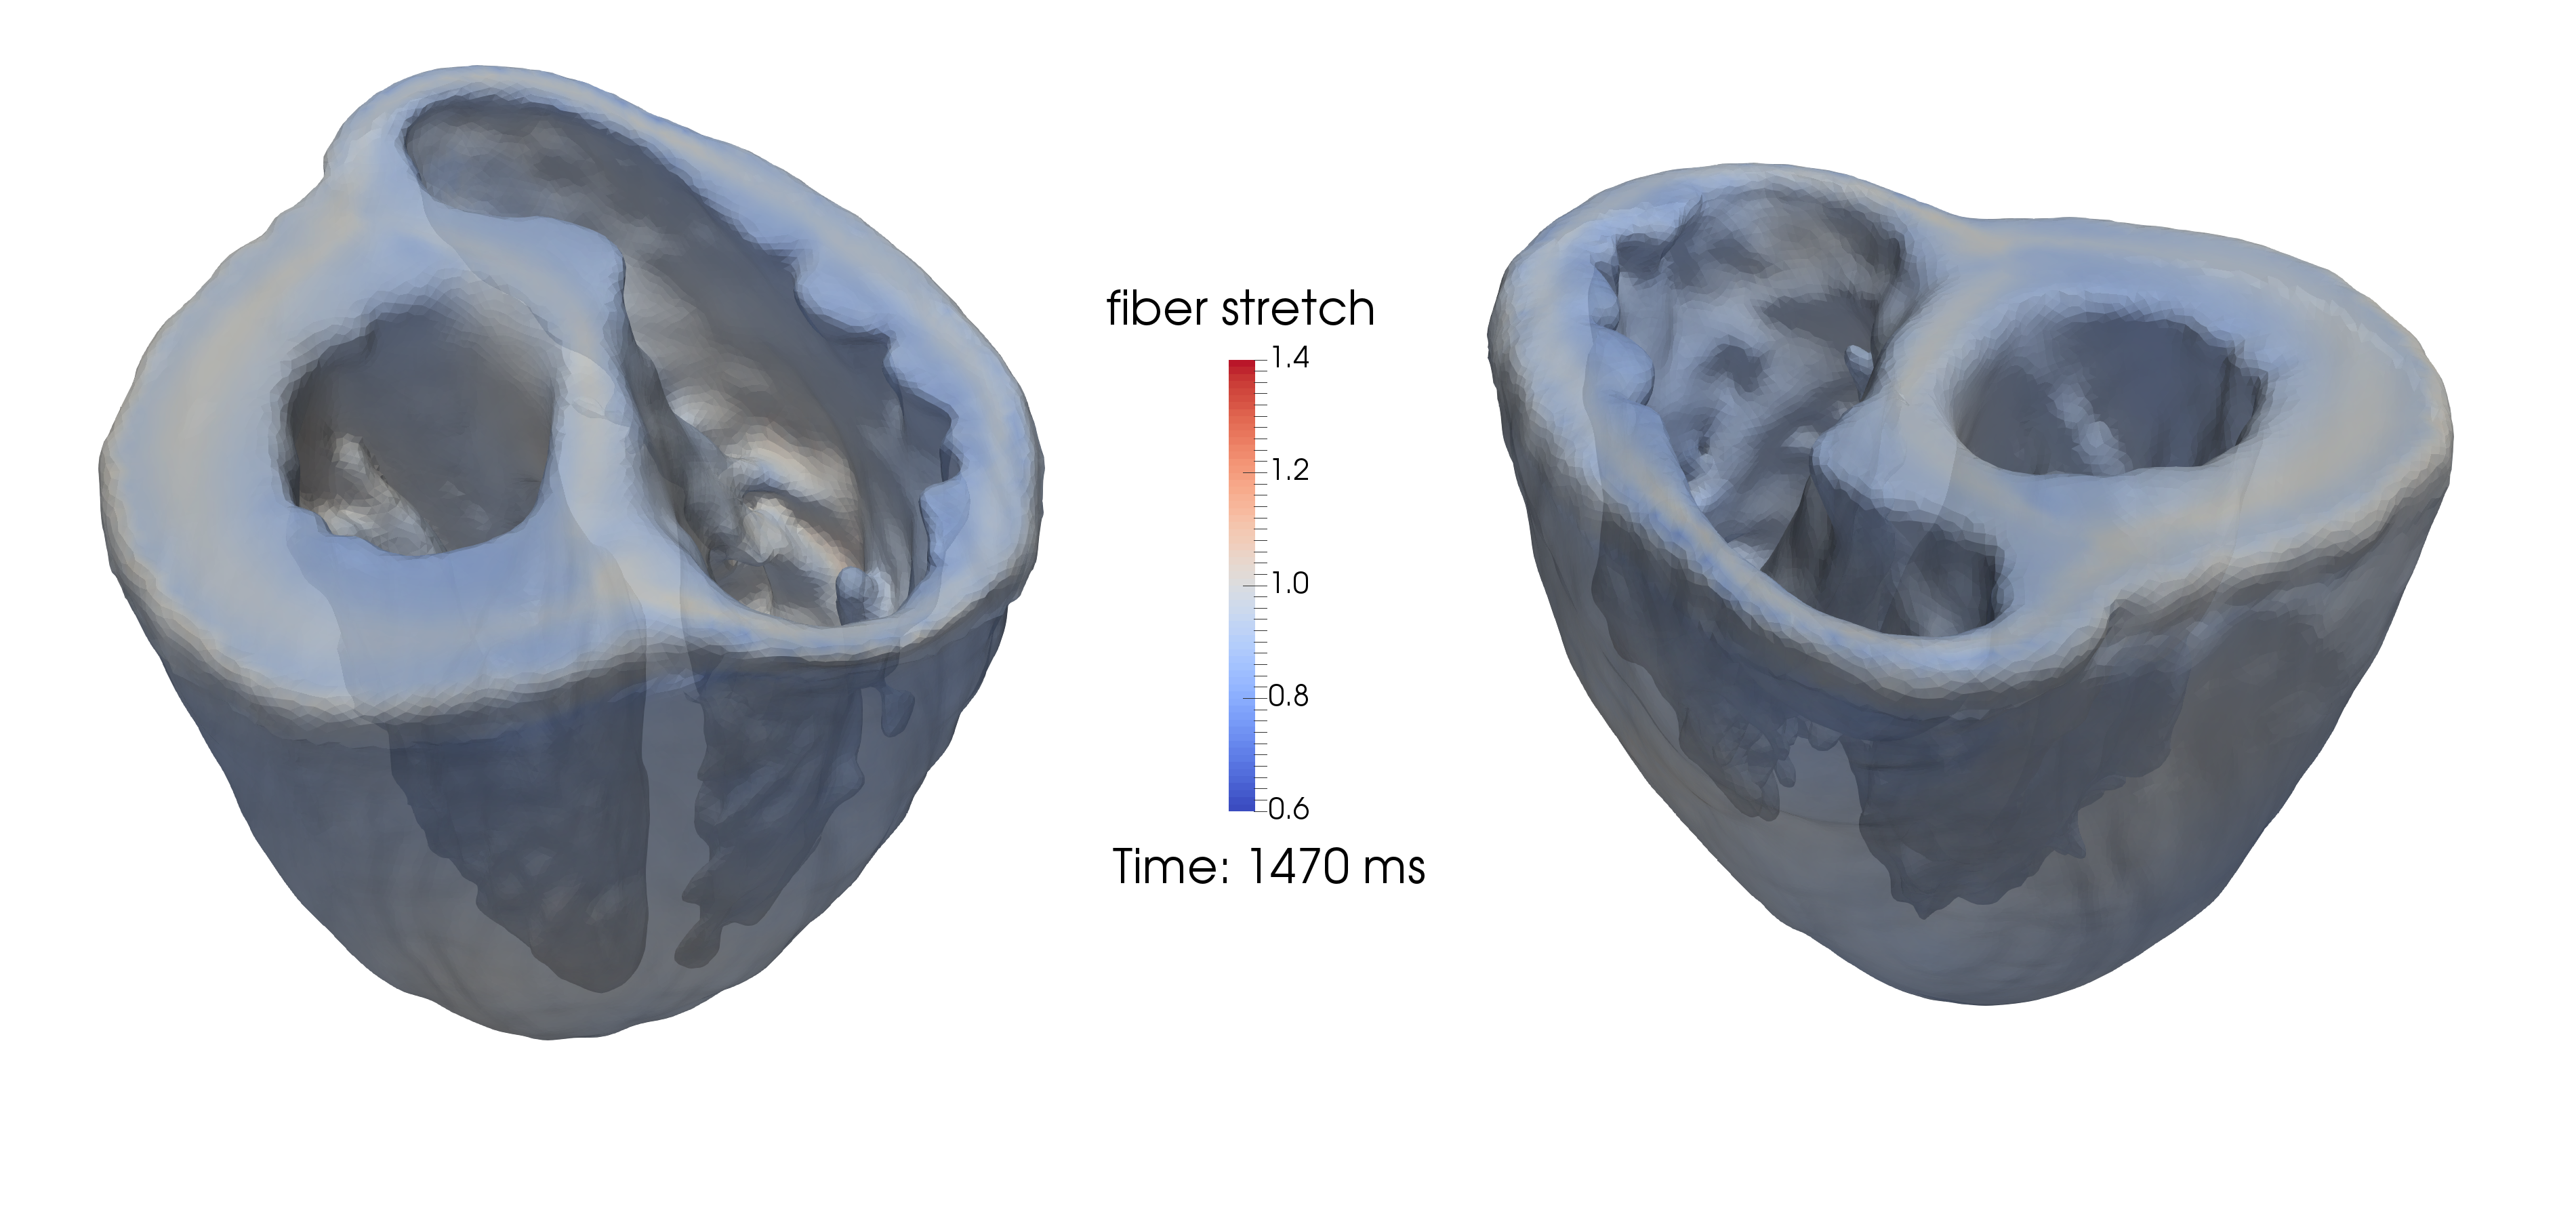
\includegraphics[scale=0.057]{media/4-cardioid/6-vid/d.png}
\label{fig:snaps4}}		
%
\caption{Deformed mesh from Cardioid simulation at different stages of cardiac cycle. Panels (a), (b), (c), and (d) correspond to the stages in the P-V loop denoted in~\figref{pv}.}
\label{fig:snaps}
\end{figure}

%%%%%%%%%%%%%%%%%%%%%%%%%%%%%%%%%%%%%%%%%%%%%%%
%%%%%%%%%%%%%%%%%%%%%%%%%%%%%%%%%%%%%%%%%%%%%%%
\section{Extension to Polyhedral Finite Elements}
\label{Polyhedral Finite Elements}

\begin{figure}[ht]
\centering
\subfigure[]{%
		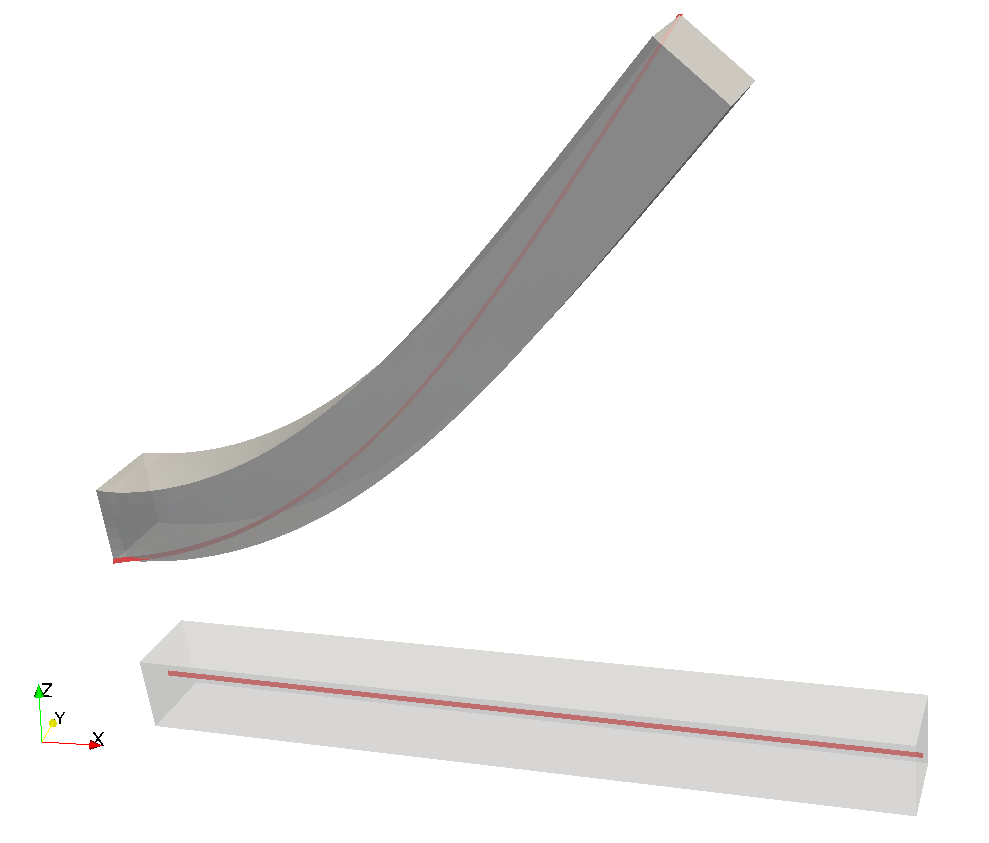
\includegraphics[scale=0.18]{media/5-verif/1-gurev2/gurev2.png}
\label{fig:beams1}}		
\subfigure[]{%
		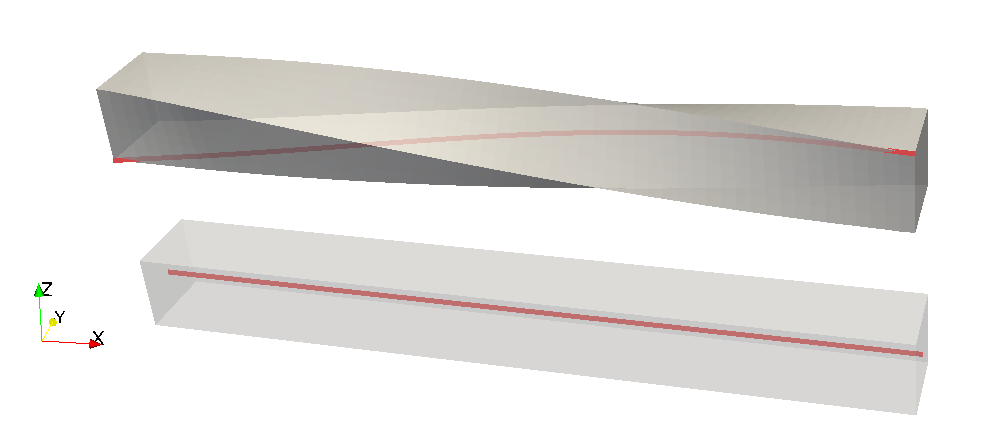
\includegraphics[scale=0.18]{media/5-verif/2-gurev3/gurev3.png}
\label{fig:beams2}}		
\subfigure[]{%
		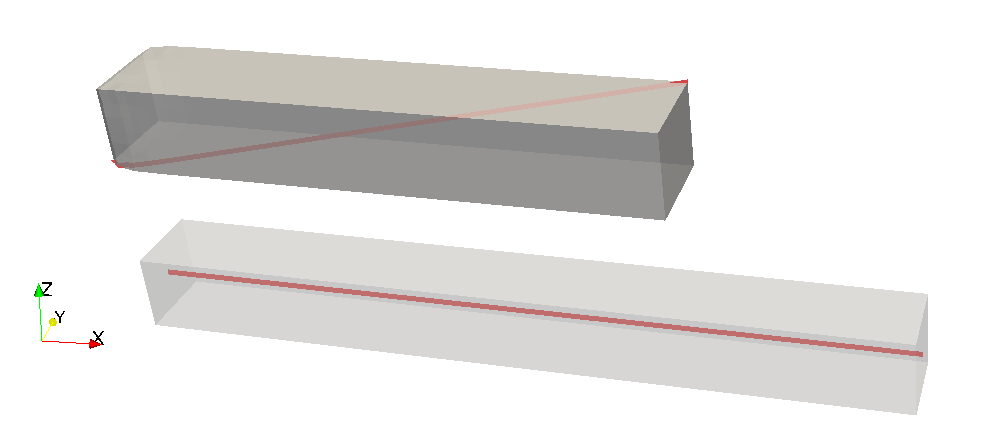
\includegraphics[scale=0.18]{media/5-verif/3-gurev4/gurev4.png}
\label{fig:beams3}}		
\subfigure[]{%
		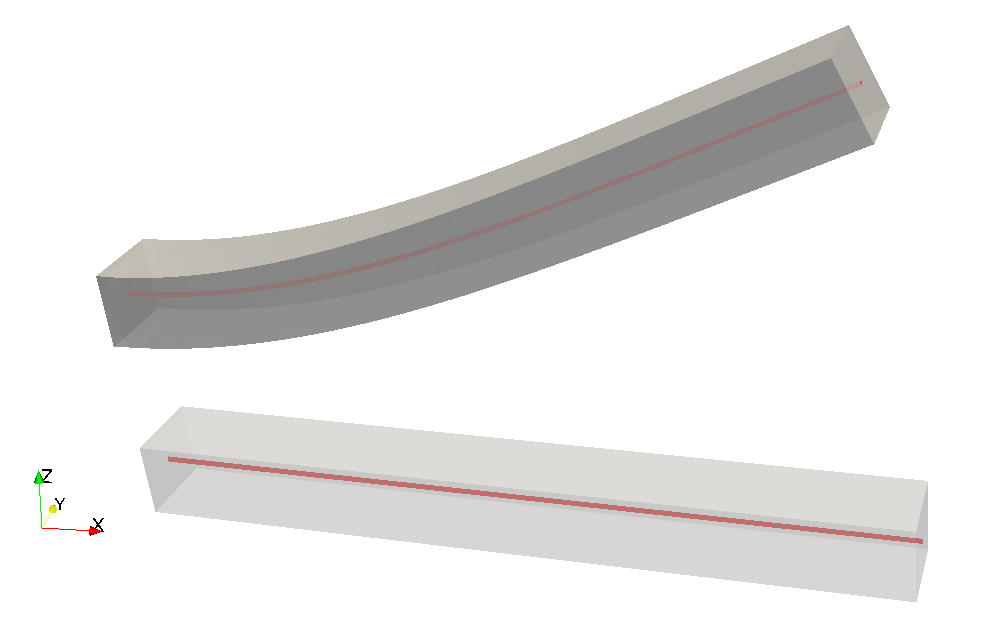
\includegraphics[scale=0.18]{media/5-verif/4-land1/land1.png}
\label{fig:beams4}}		
%
\caption{Undeformed (bottom) and deformed (top) configurations for cantilever beam verification problems: (a) Gurev P2: bending, (b) Gurev P3: torsion, c) Gurev P4: active contraction, and (d) Land P1: bending. The red curve denotes the curve over which displacements and positions are recorded for comparison of results.}
\label{fig:beams}
\end{figure}

\begin{figure}[ht]
\centering
\subfigure[]{%
		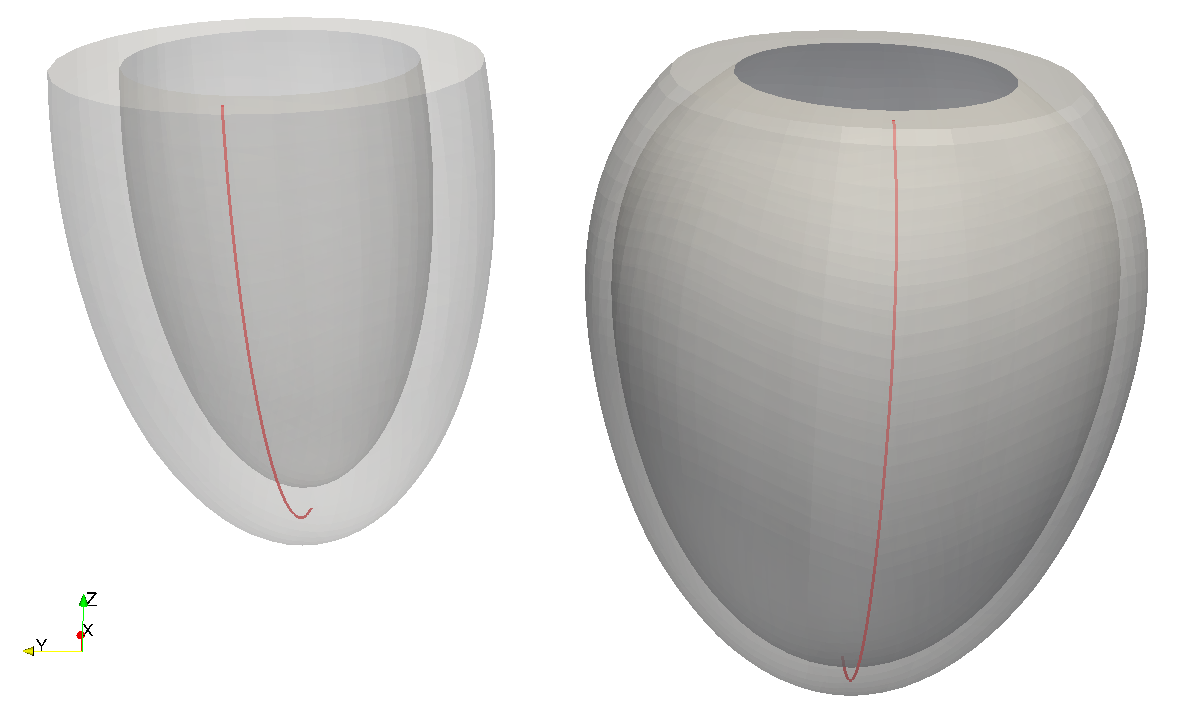
\includegraphics[scale=0.18]{media/5-verif/5-land2/land2-1.png}
\label{fig:ventricles1}}		
\subfigure[]{%
		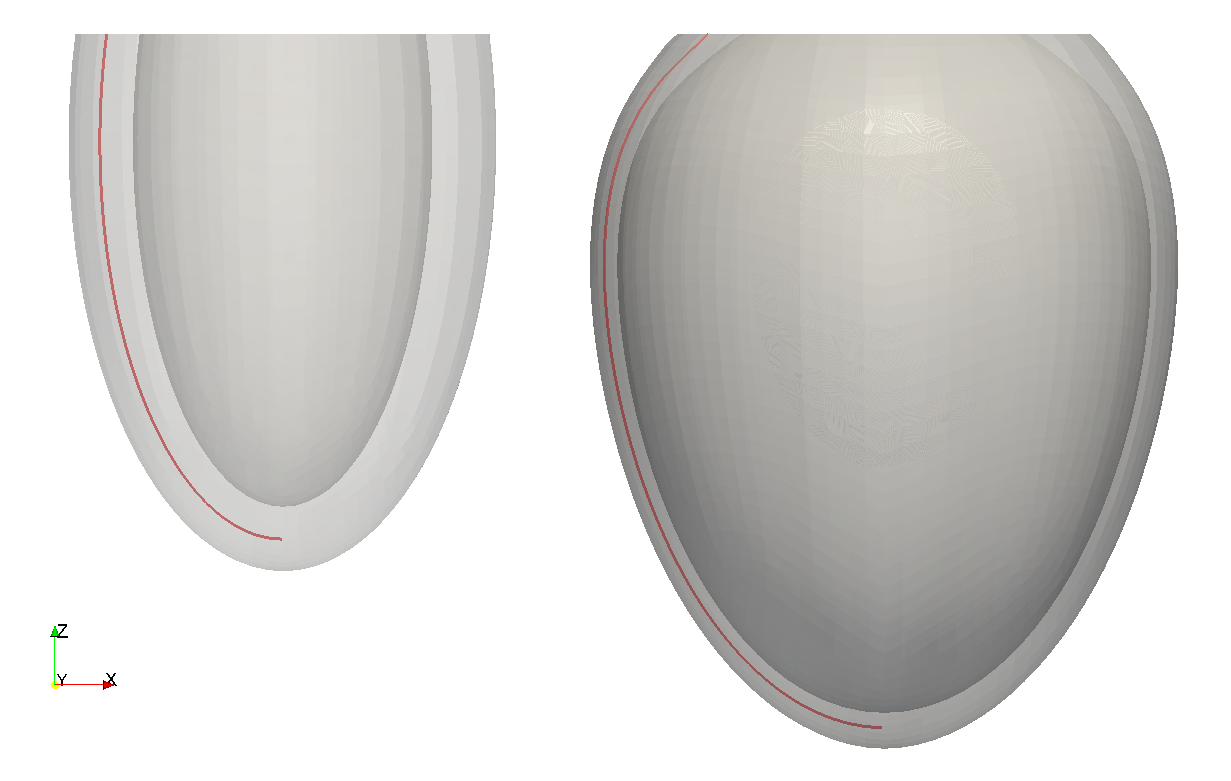
\includegraphics[scale=0.18]{media/5-verif/5-land2/land2-2.png}
\label{fig:ventricles2}}		
\subfigure[]{%
		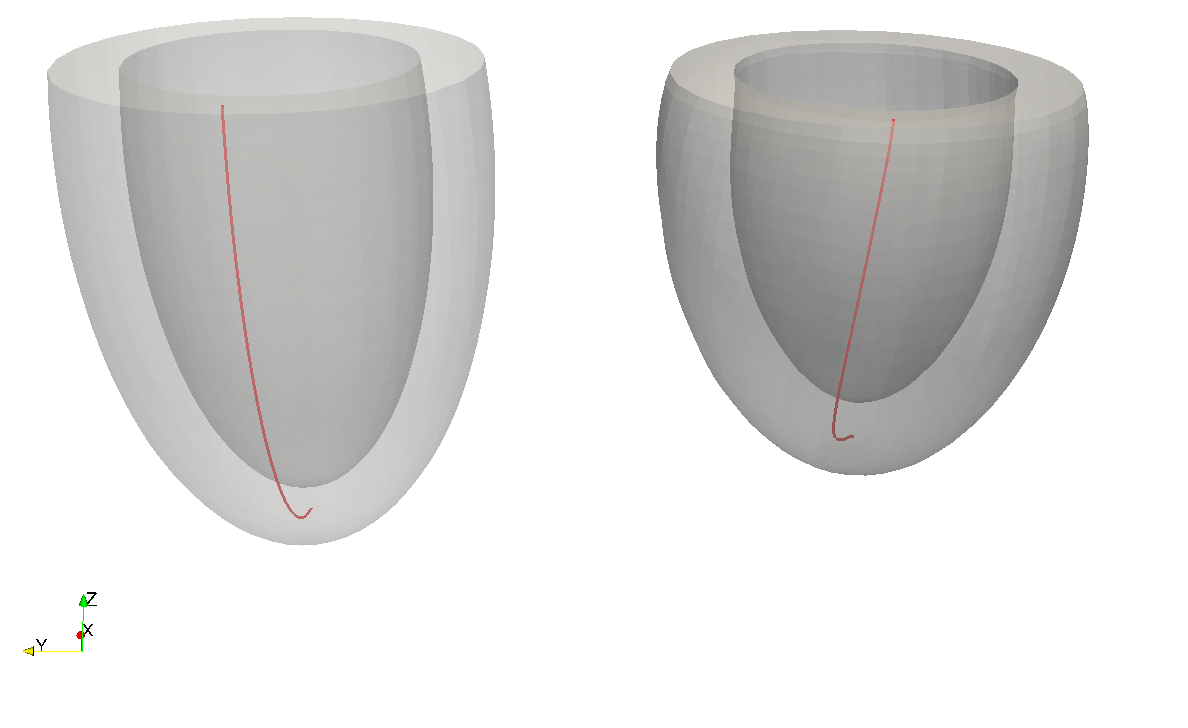
\includegraphics[scale=0.18]{media/5-verif/6-land3/land3-1.png}
\label{fig:ventricles3}}		
\subfigure[]{%
		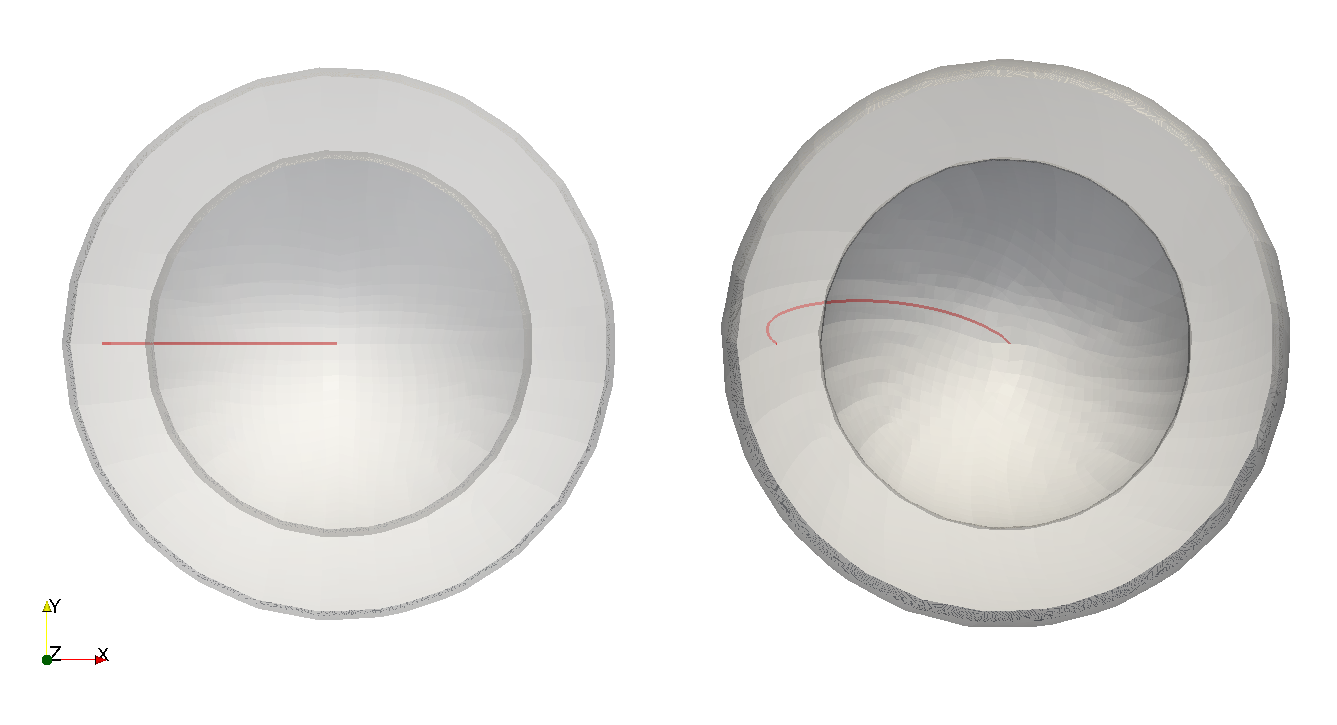
\includegraphics[scale=0.16]{media/5-verif/6-land3/land3-2.png}
\label{fig:ventricles4}}		
%
\caption{Undeformed (left) and deformed (right) configurations for single ventricle verification problems: (a,b) Land P2: inflation, and (c,d) Land P3: inflation and active contraction. The red curve denotes the curve over which displacements and positions are recorded for comparison of results.}
\label{fig:ventricles}
\end{figure}

\begin{figure}[ht]
\centering
\subfigure[]{%
		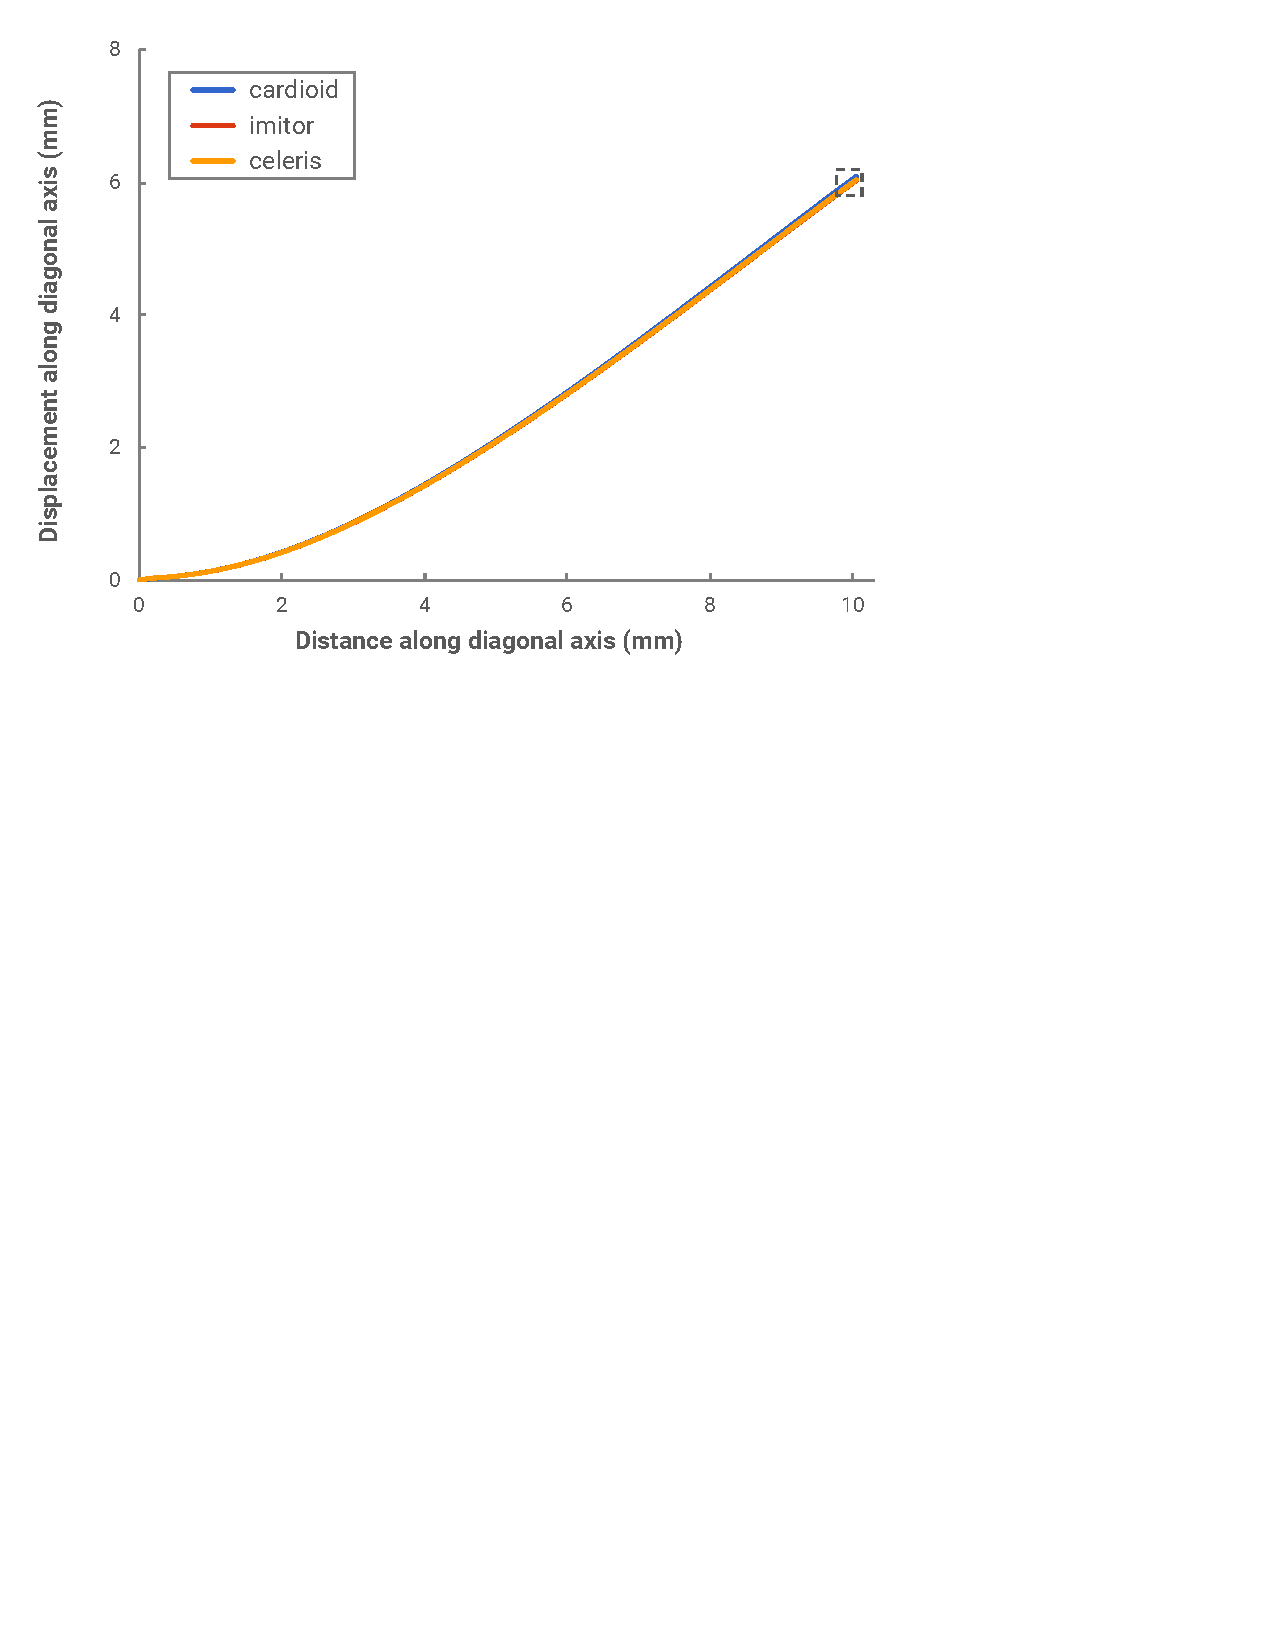
\includegraphics[scale=0.48]{media/5-verif/1-gurev2/gurev2-1.pdf}
\label{fig:gurev2-1}}		
\subfigure[]{%
		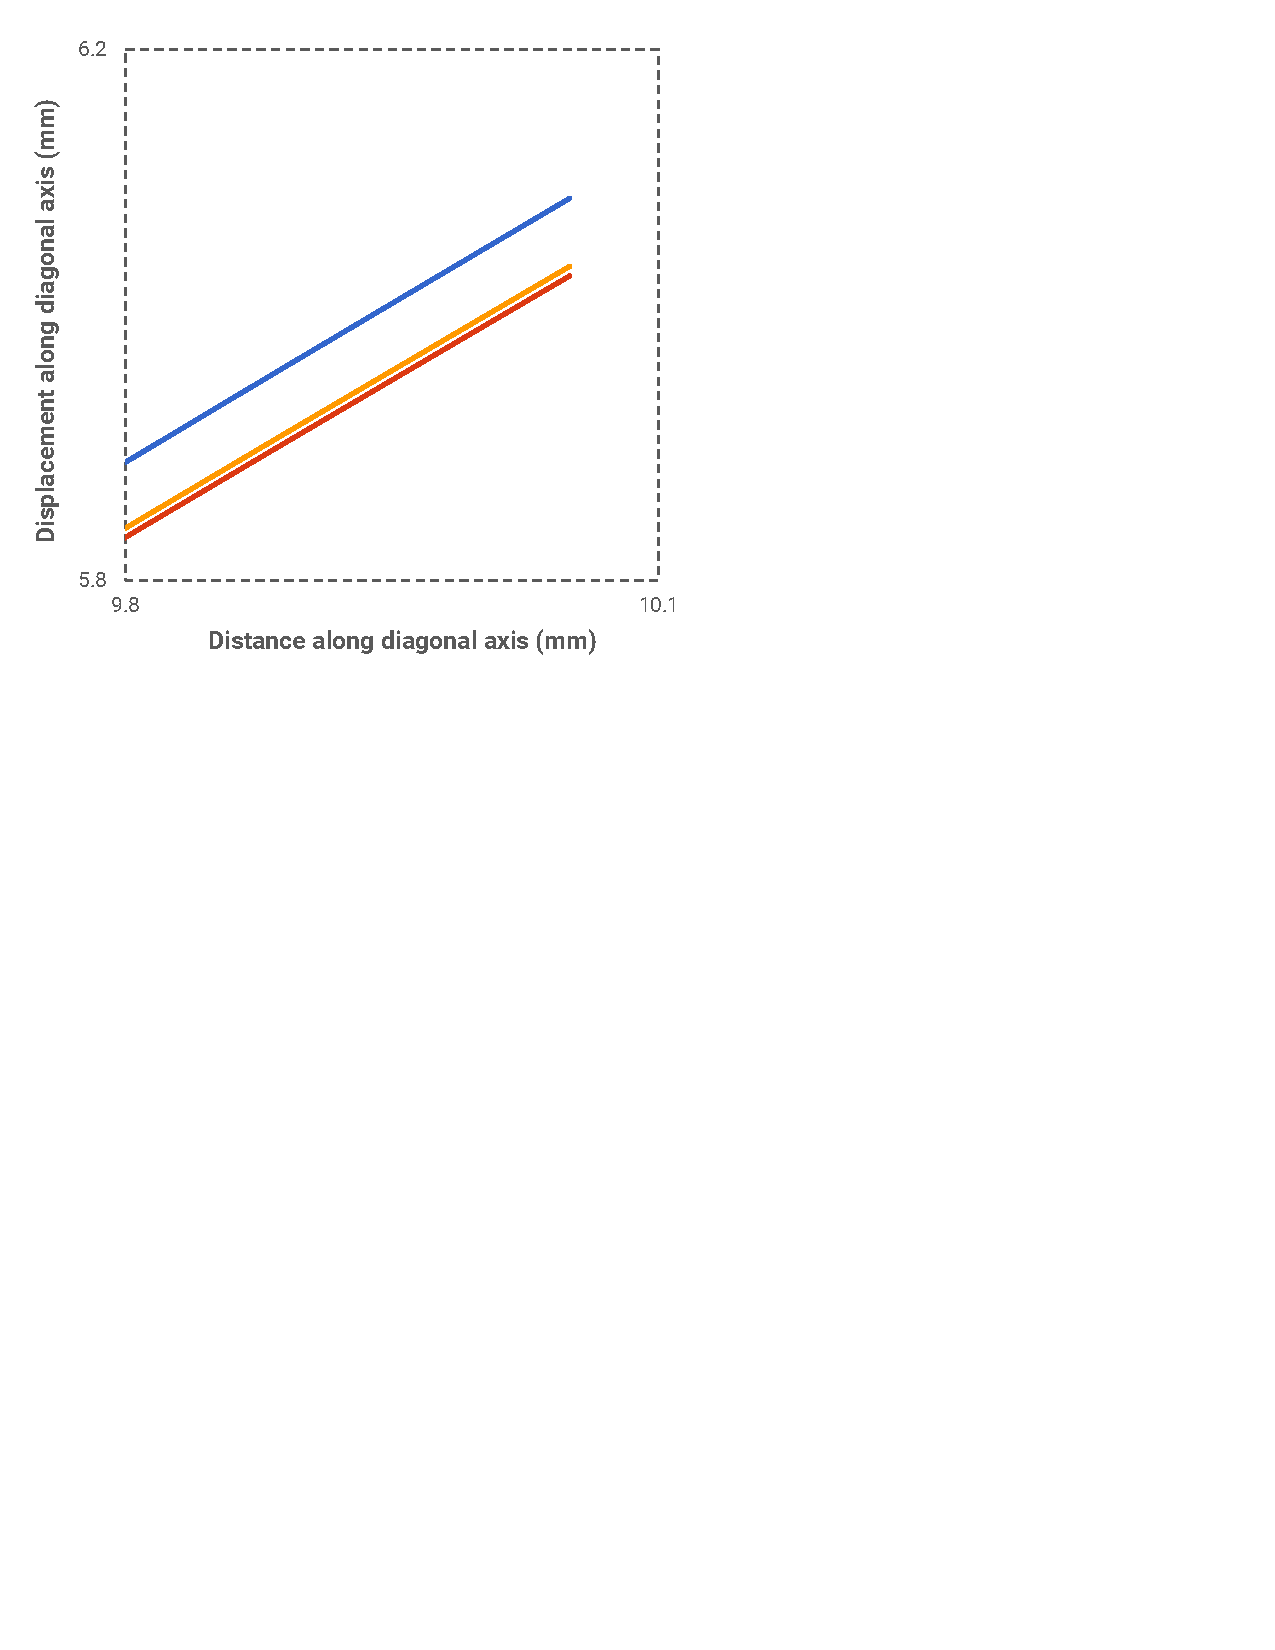
\includegraphics[scale=0.48]{media/5-verif/1-gurev2/gurev2-2.pdf}
\label{fig:gurev2-2}}		
%
\caption{Results for Gurev P2 verification problem: (a) Displacement magnitude along diagonal axis, with (b) details for the free end of the beam}
\label{fig:gurev2}
\end{figure}

\begin{figure}[ht!]
\centering
\subfigure[]{%
		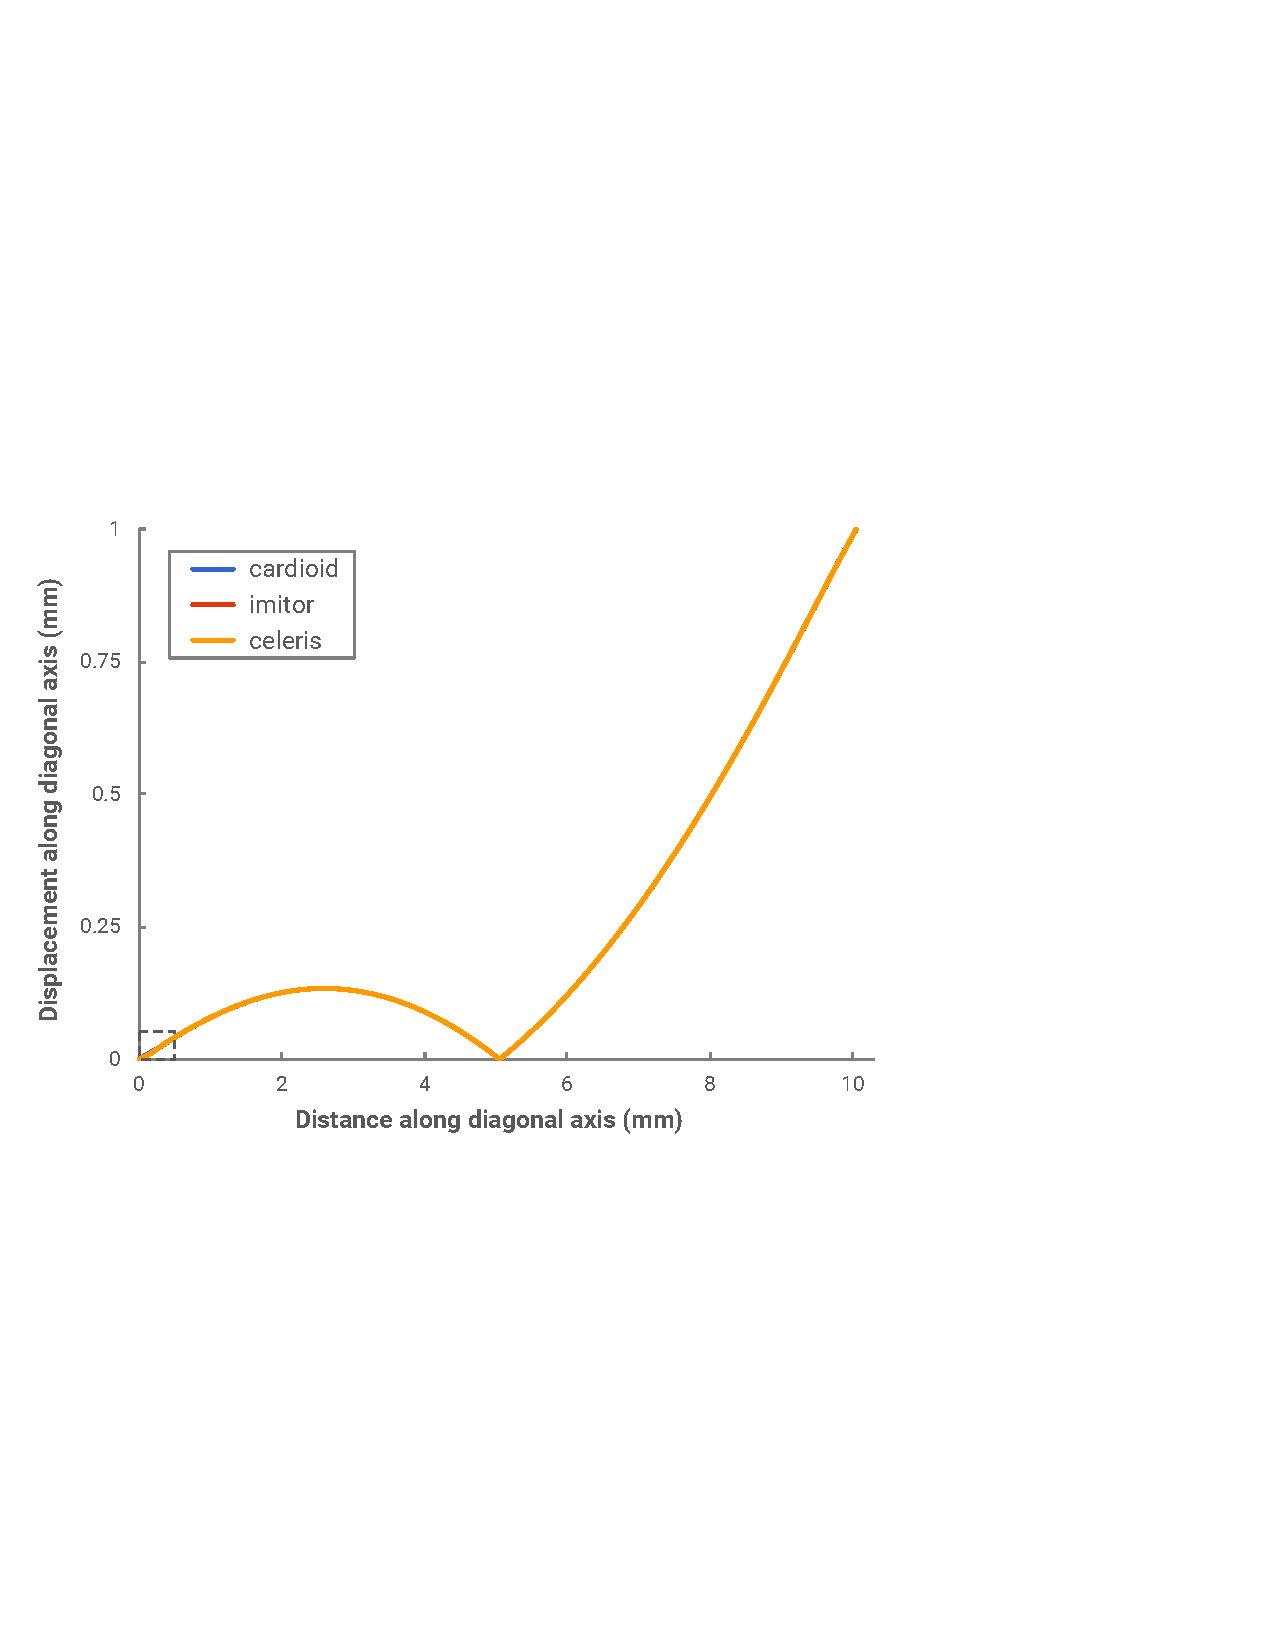
\includegraphics[scale=0.48]{media/5-verif/2-gurev3/gurev3-1.pdf}
\label{fig:gurev3-1}}		
\subfigure[]{%
		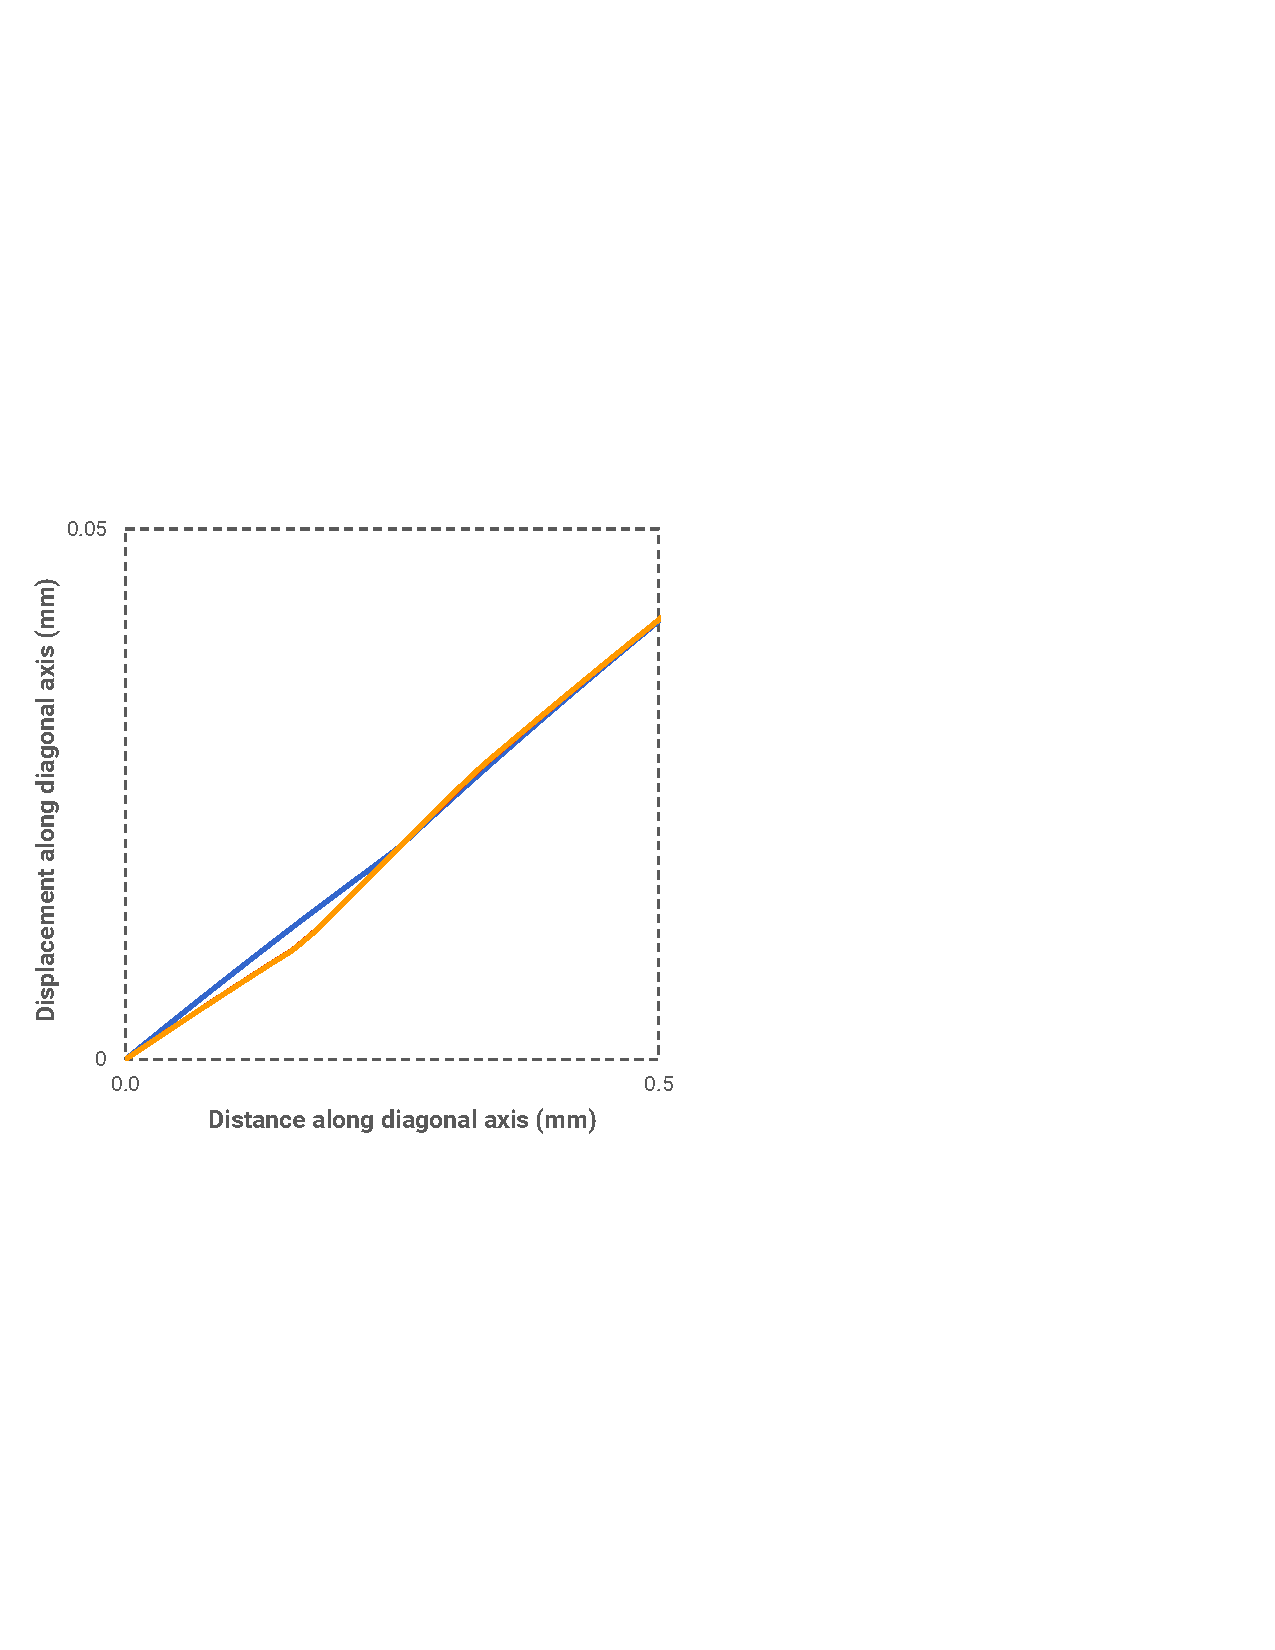
\includegraphics[scale=0.48]{media/5-verif/2-gurev3/gurev3-2.pdf}
\label{fig:gure3-2}}		
%
\caption{Results for Gurev P3 verification problem: (a) Displacement magnitude along diagonal axis, with (b) details for the fixed end of the beam. The results for imitor and Celeris are indistinguishable in these plots.}
\label{fig:gurev3}
\end{figure}

\begin{figure}[ht!]
\centering
\subfigure[]{%
		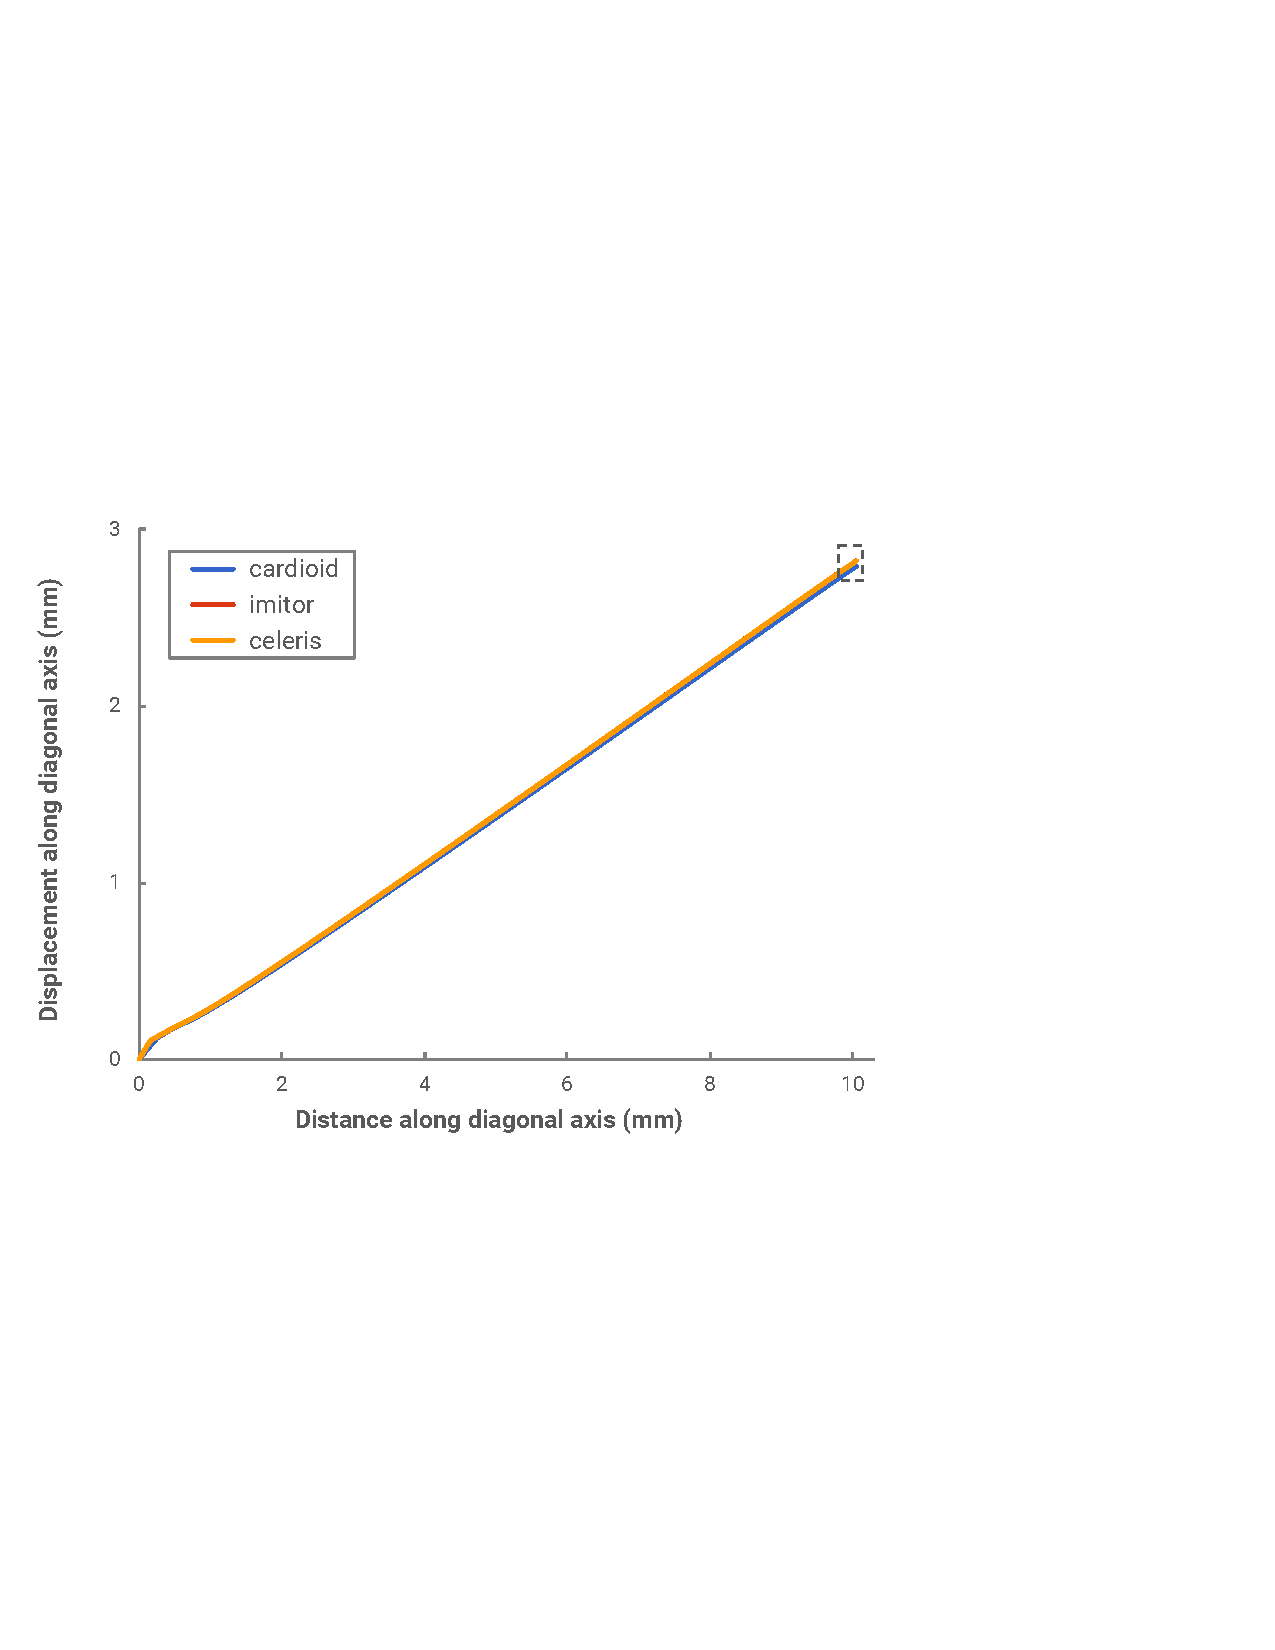
\includegraphics[scale=0.48]{media/5-verif/3-gurev4/gurev4-1.pdf}
\label{fig:gurev4-1}}		
\subfigure[]{%
		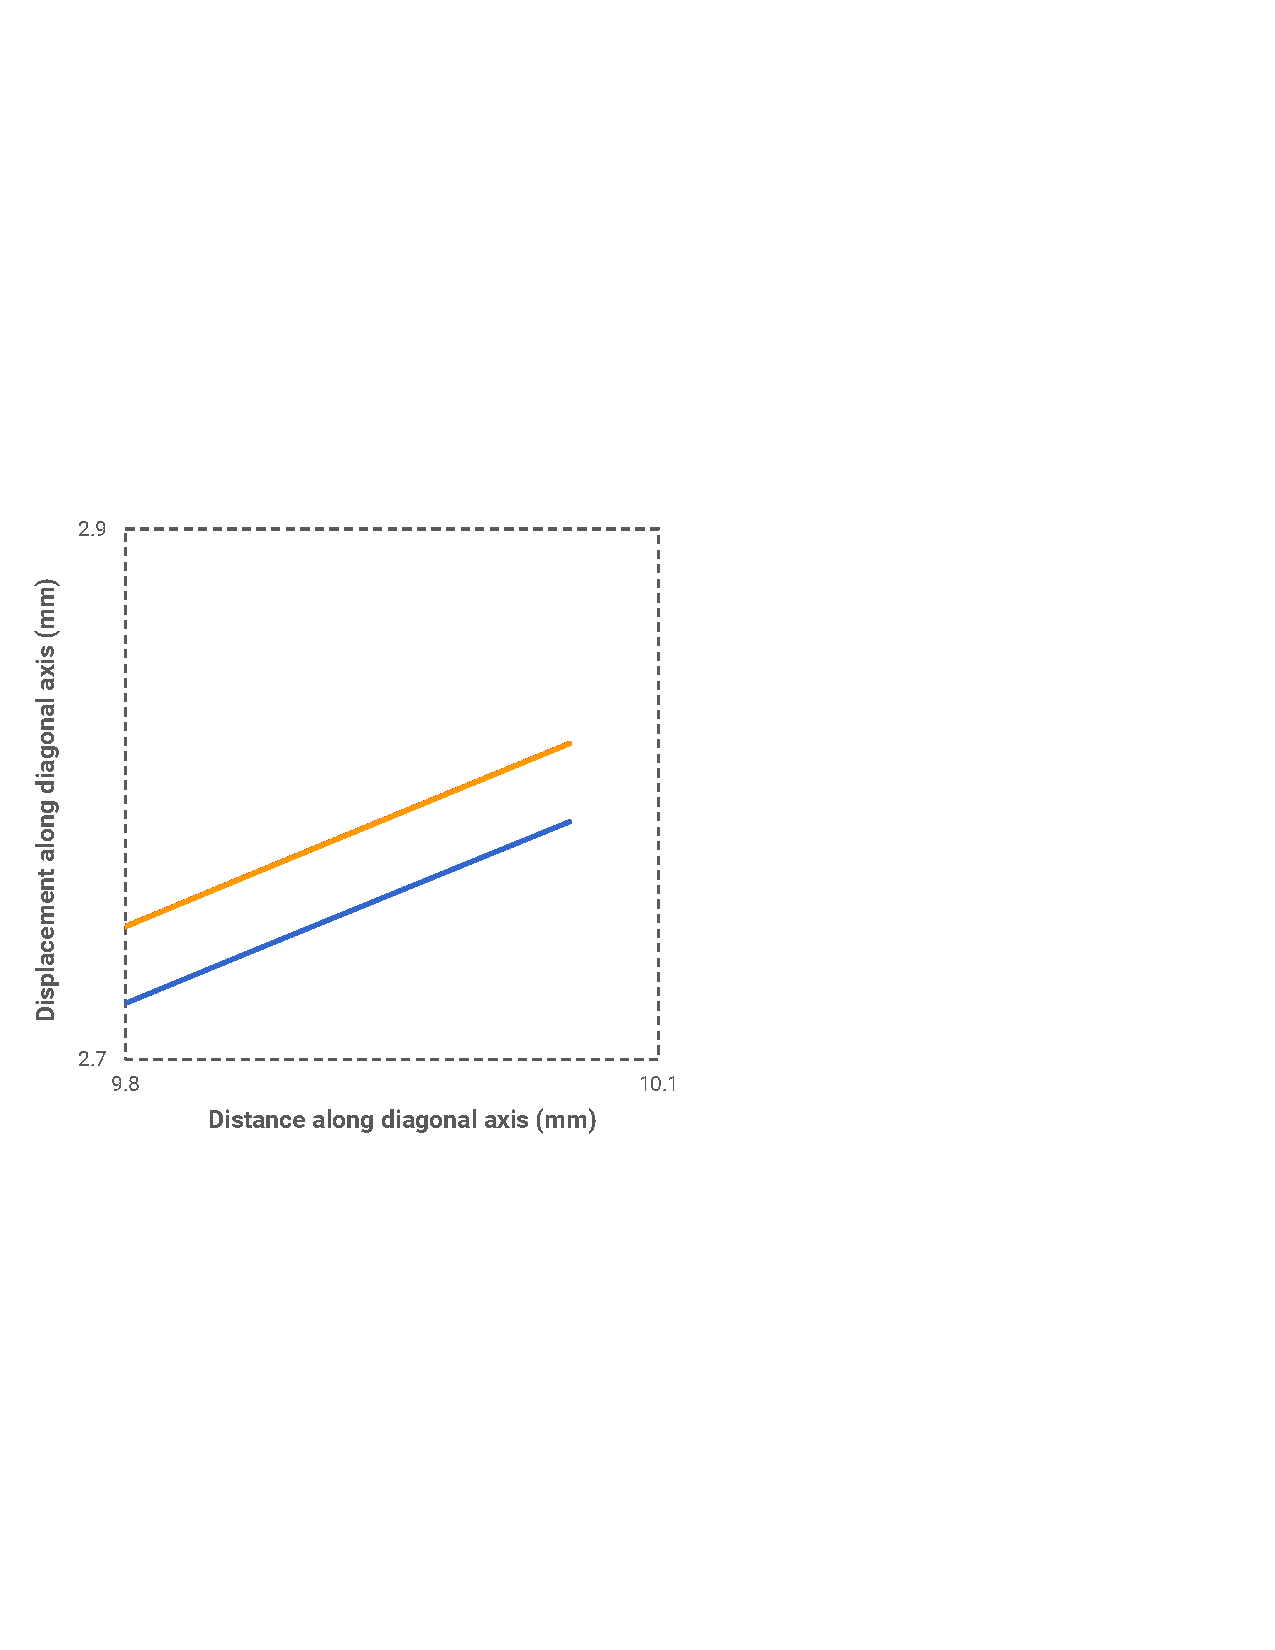
\includegraphics[scale=0.48]{media/5-verif/3-gurev4/gurev4-2.pdf}
\label{fig:gurev4-2}}		
%
\caption{Results for Gurev P4 verification problem: (a) Displacement magnitude along diagonal axis, with (b) details for the free end of the beam. The results for imitor and Celeris are indistinguishable in these plots.}
\label{fig:gurev4}
\end{figure}

\begin{figure}[ht!]
\centering
\subfigure[]{%
		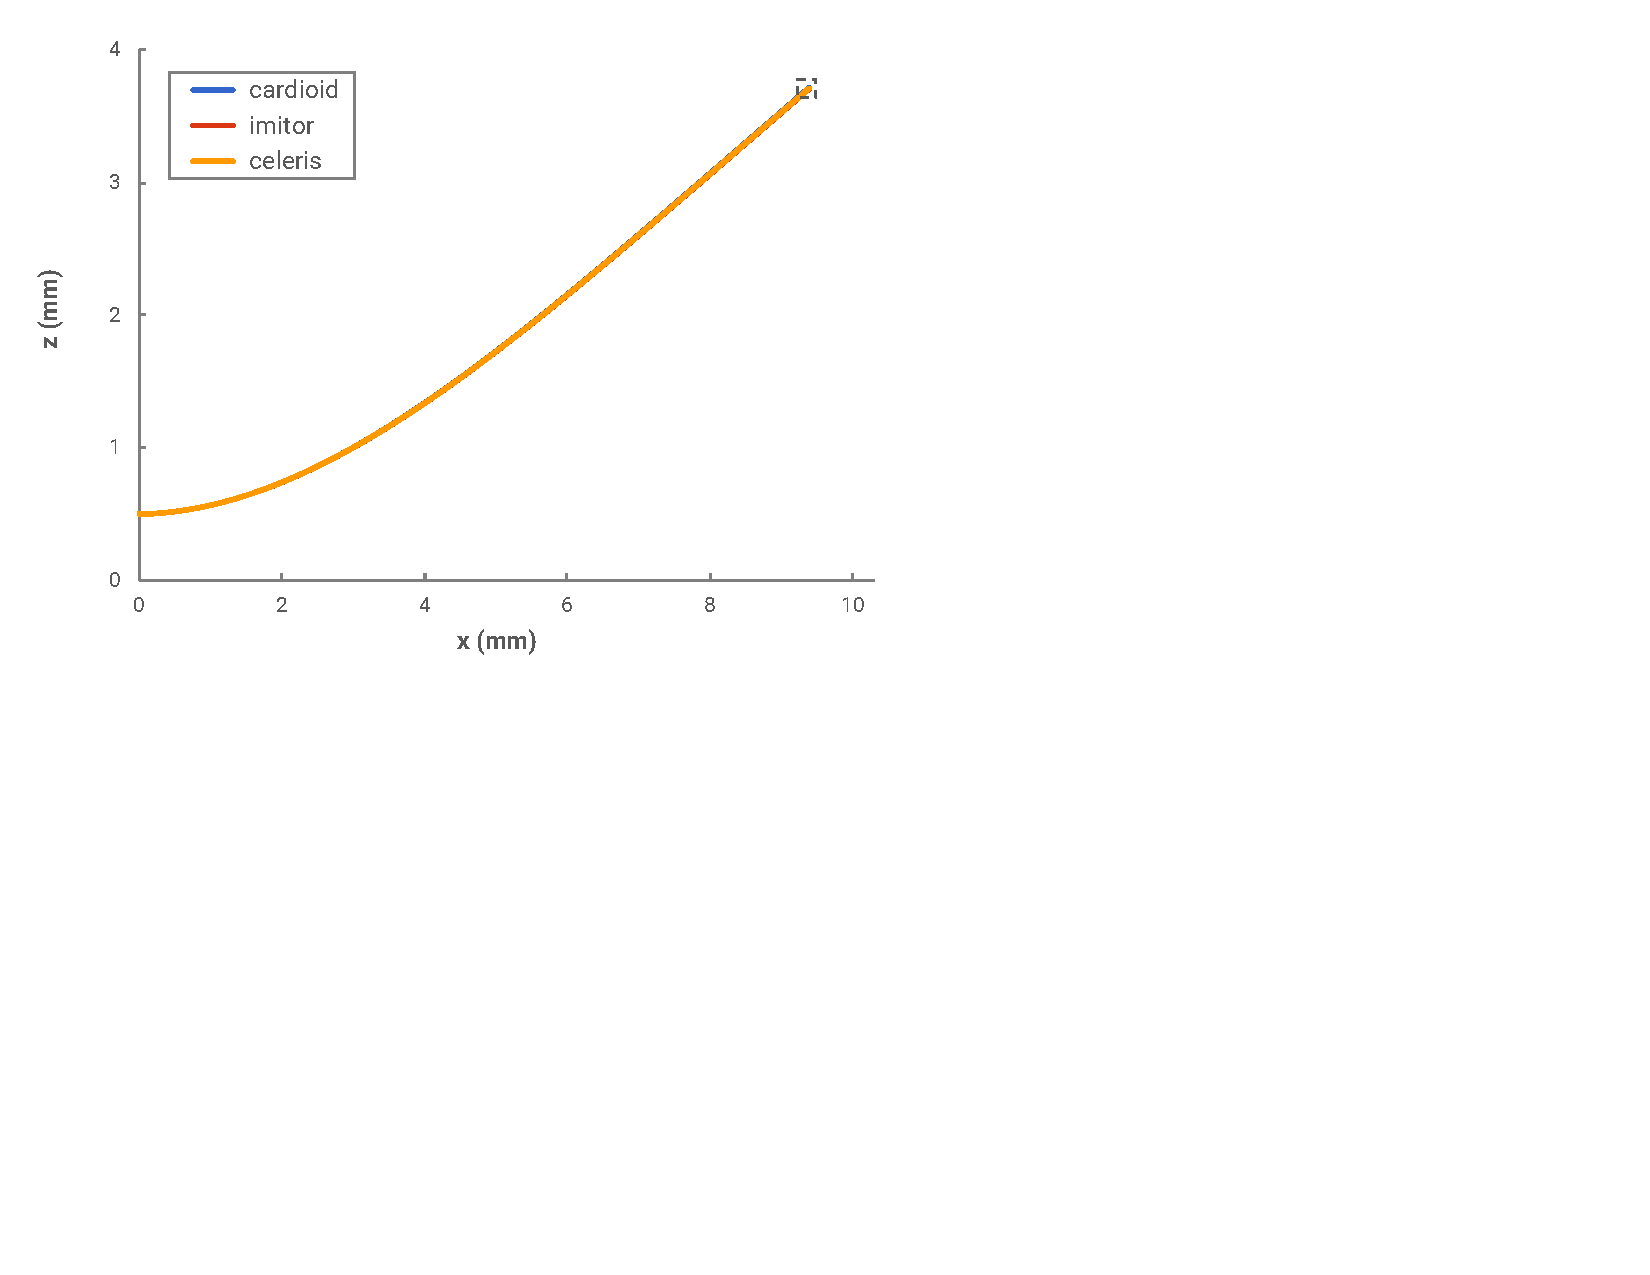
\includegraphics[scale=0.48]{media/5-verif/4-land1/land1-1.pdf}
\label{fig:land1-1}}		
\subfigure[]{%
		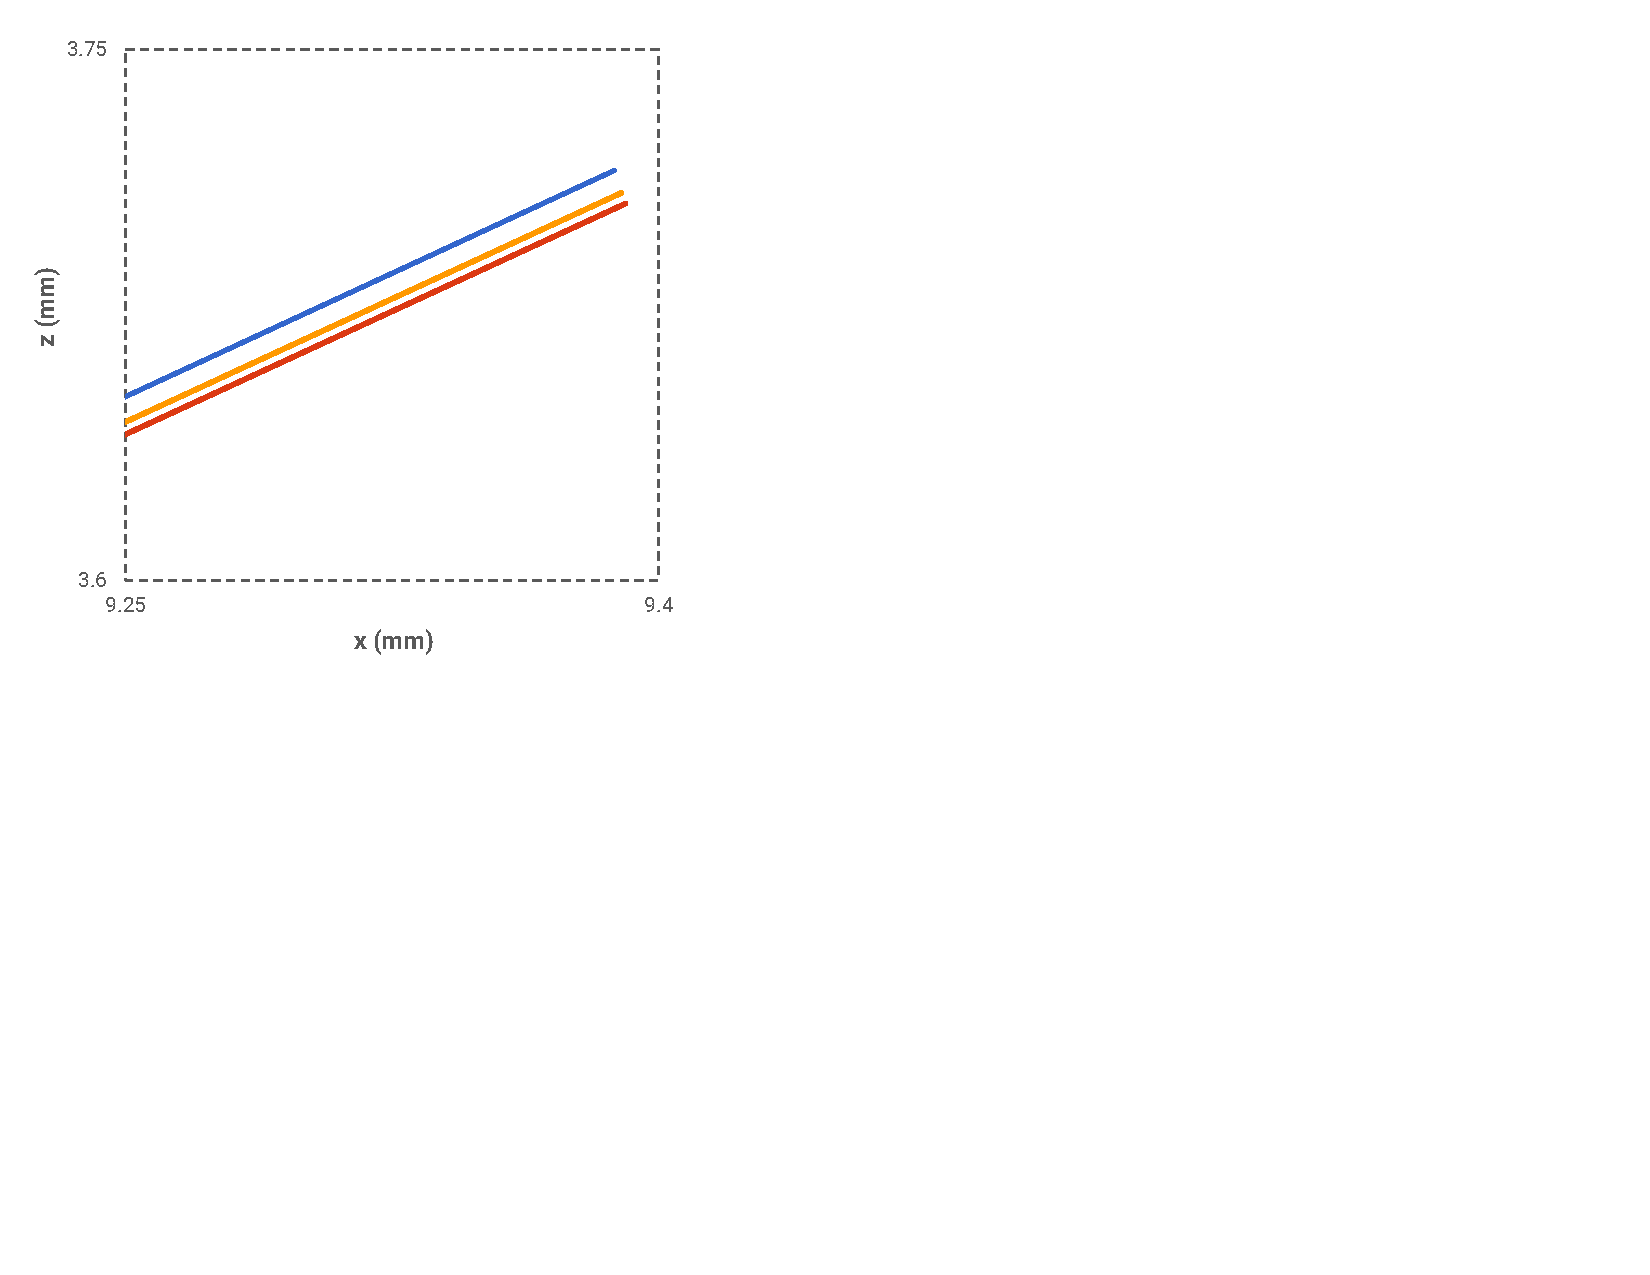
\includegraphics[scale=0.48]{media/5-verif/4-land1/land1-2.pdf}
\label{fig:land1-2}}	
\subfigure[]{%
		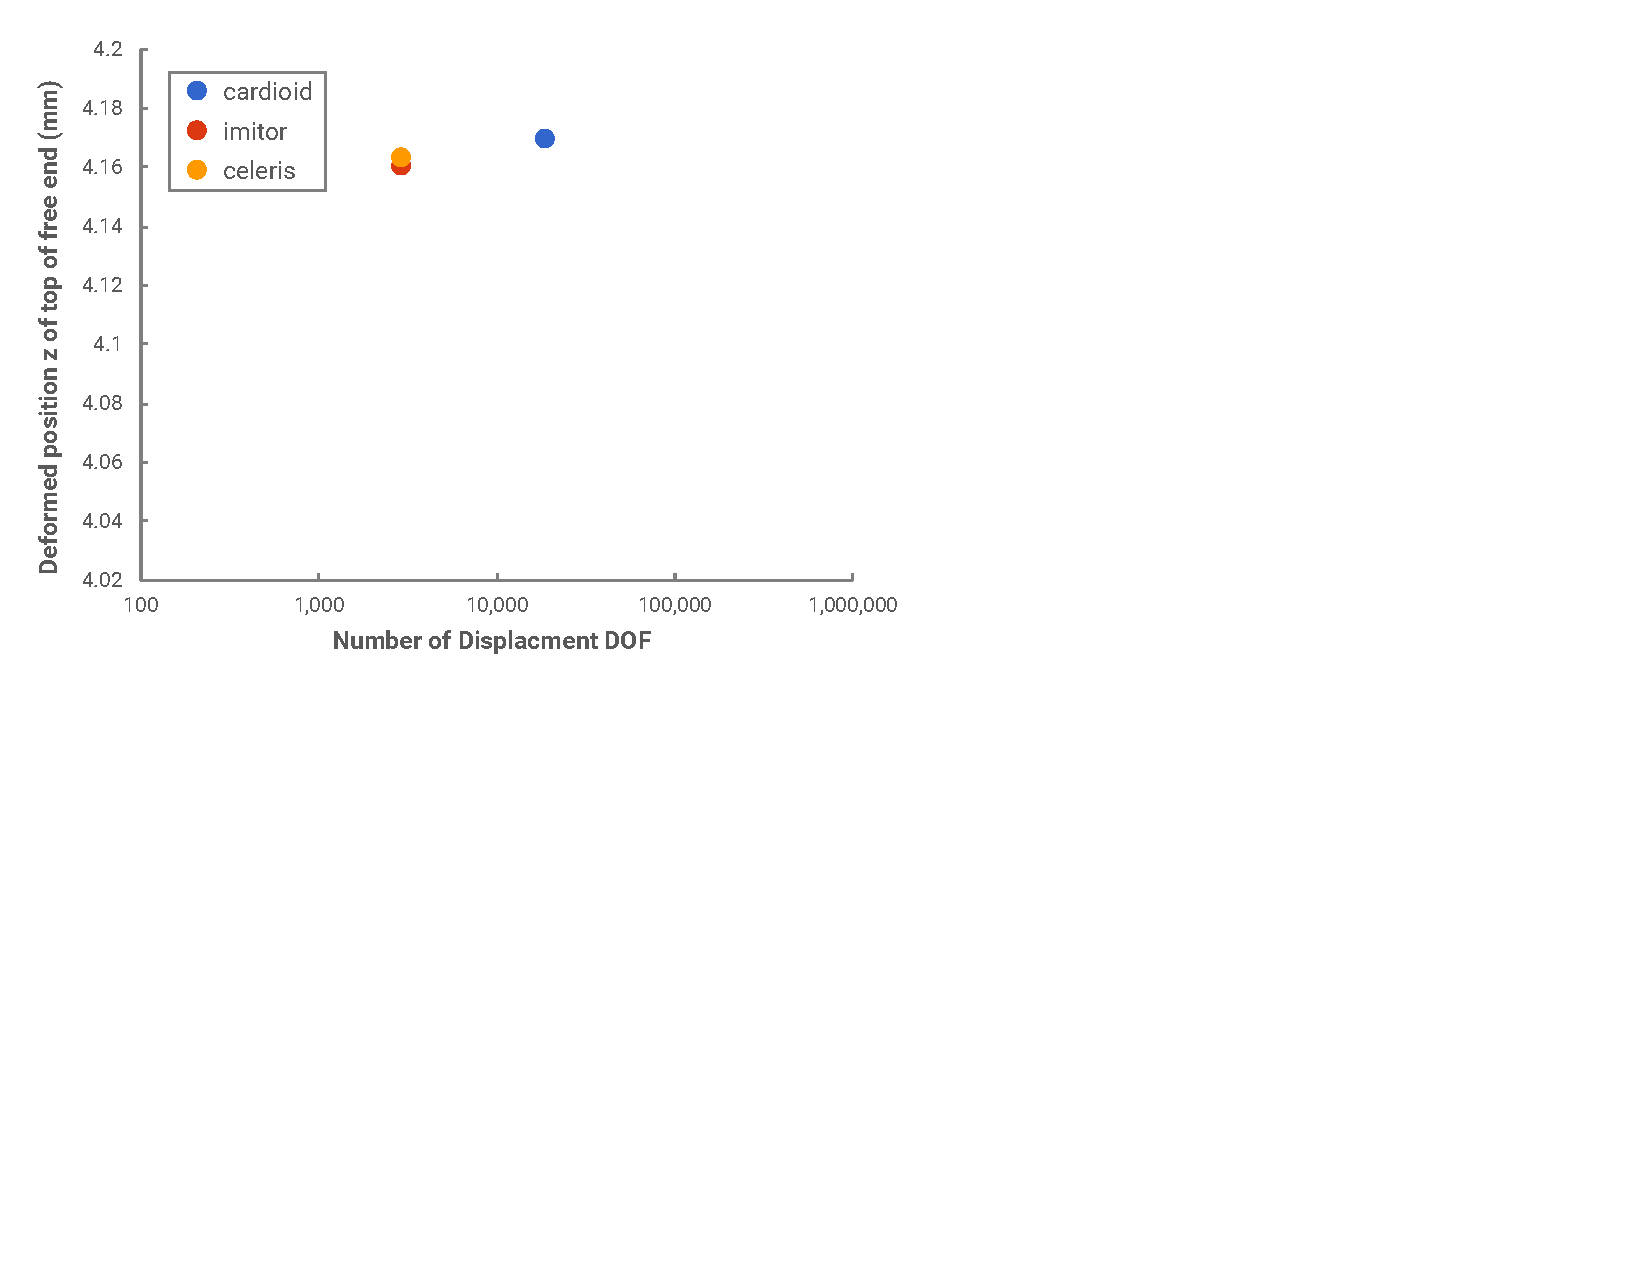
\includegraphics[scale=0.48]{media/5-verif/4-land1/land1-3.pdf}
\label{fig:land1-3}}			
%
\caption{Results for Land P1 verification problem: (a) Deformed position of midline, with (b) details for the free end of the beam. Panel (c) shows the deformed position of the point $\mathbf{X} = (10, 0.5, 1)$ for each of the simulation codes.}
\label{fig:land1}
\end{figure}


\begin{figure}[ht!]
\centering
\subfigure[]{%
		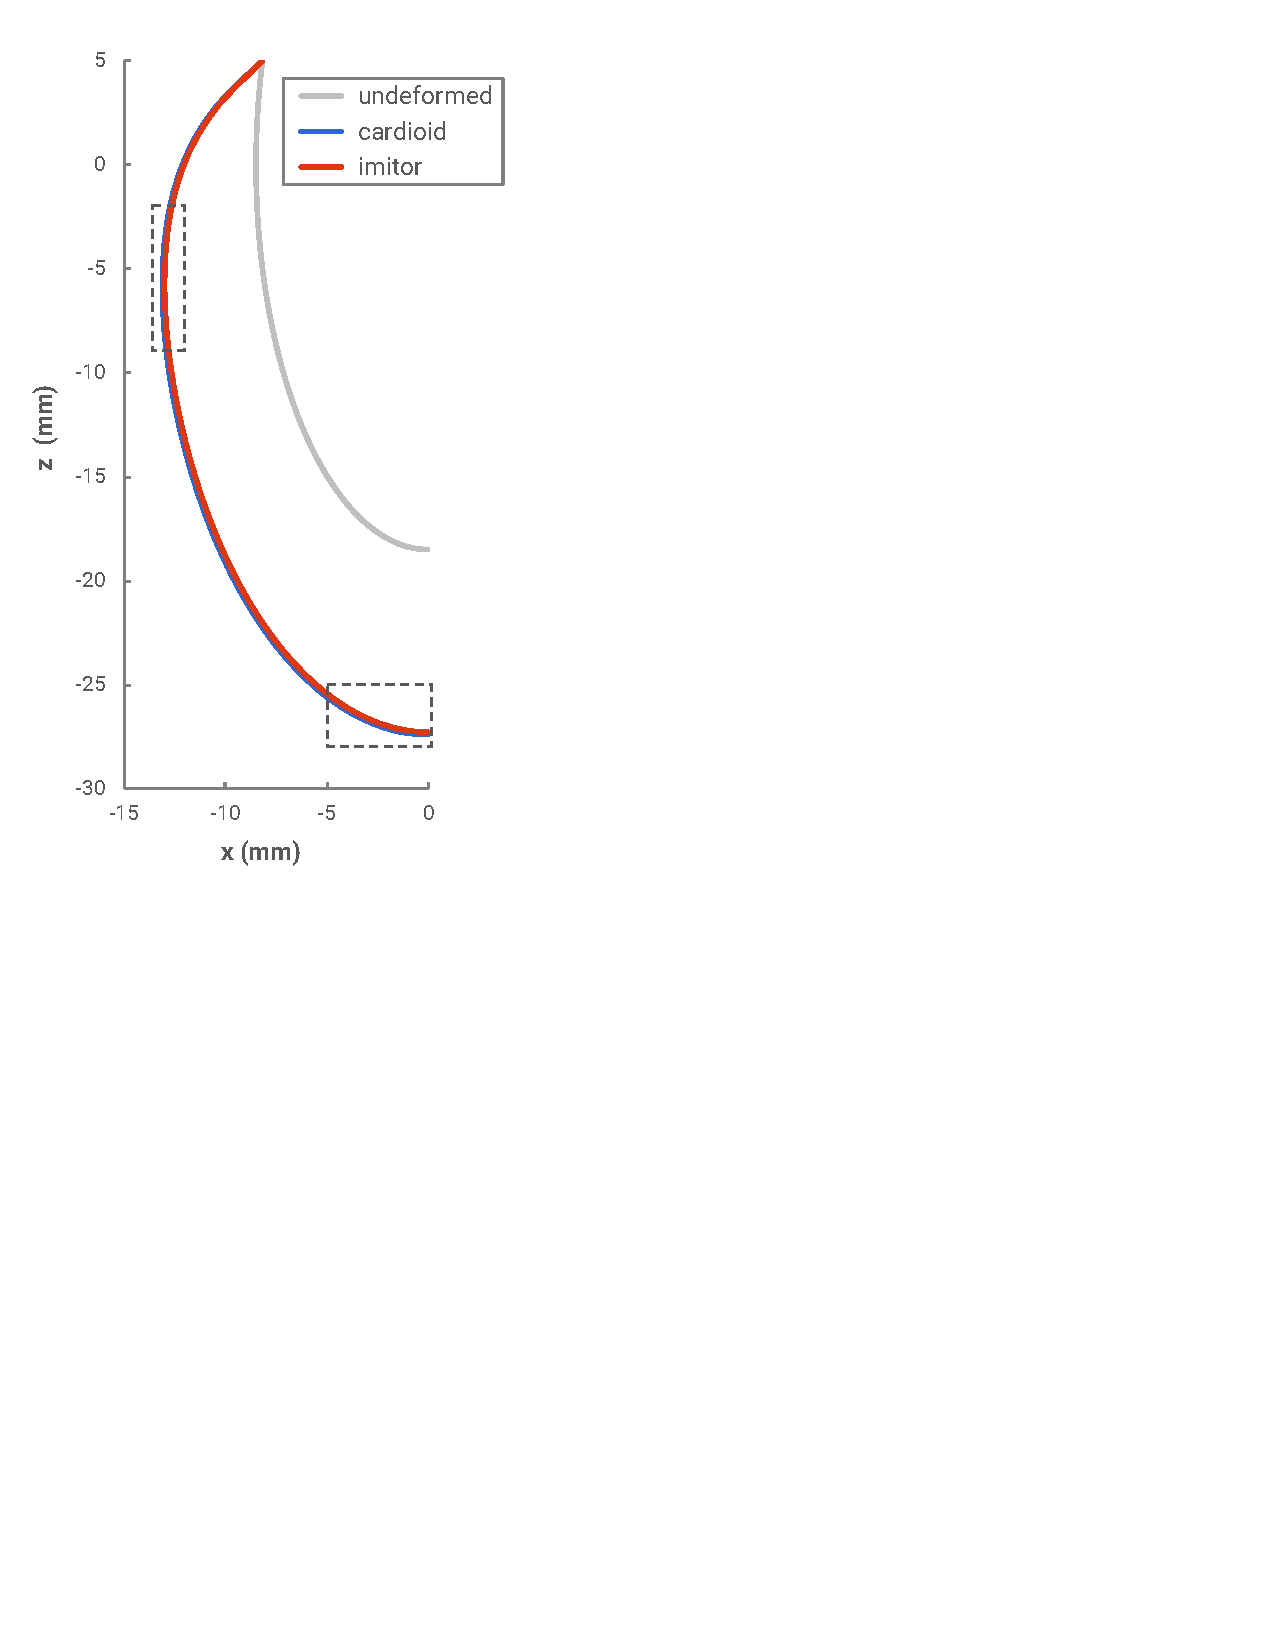
\includegraphics[scale=0.48]{media/5-verif/5-land2/land2-1.pdf}
\label{fig:land2-1}}		
\subfigure[]{%
		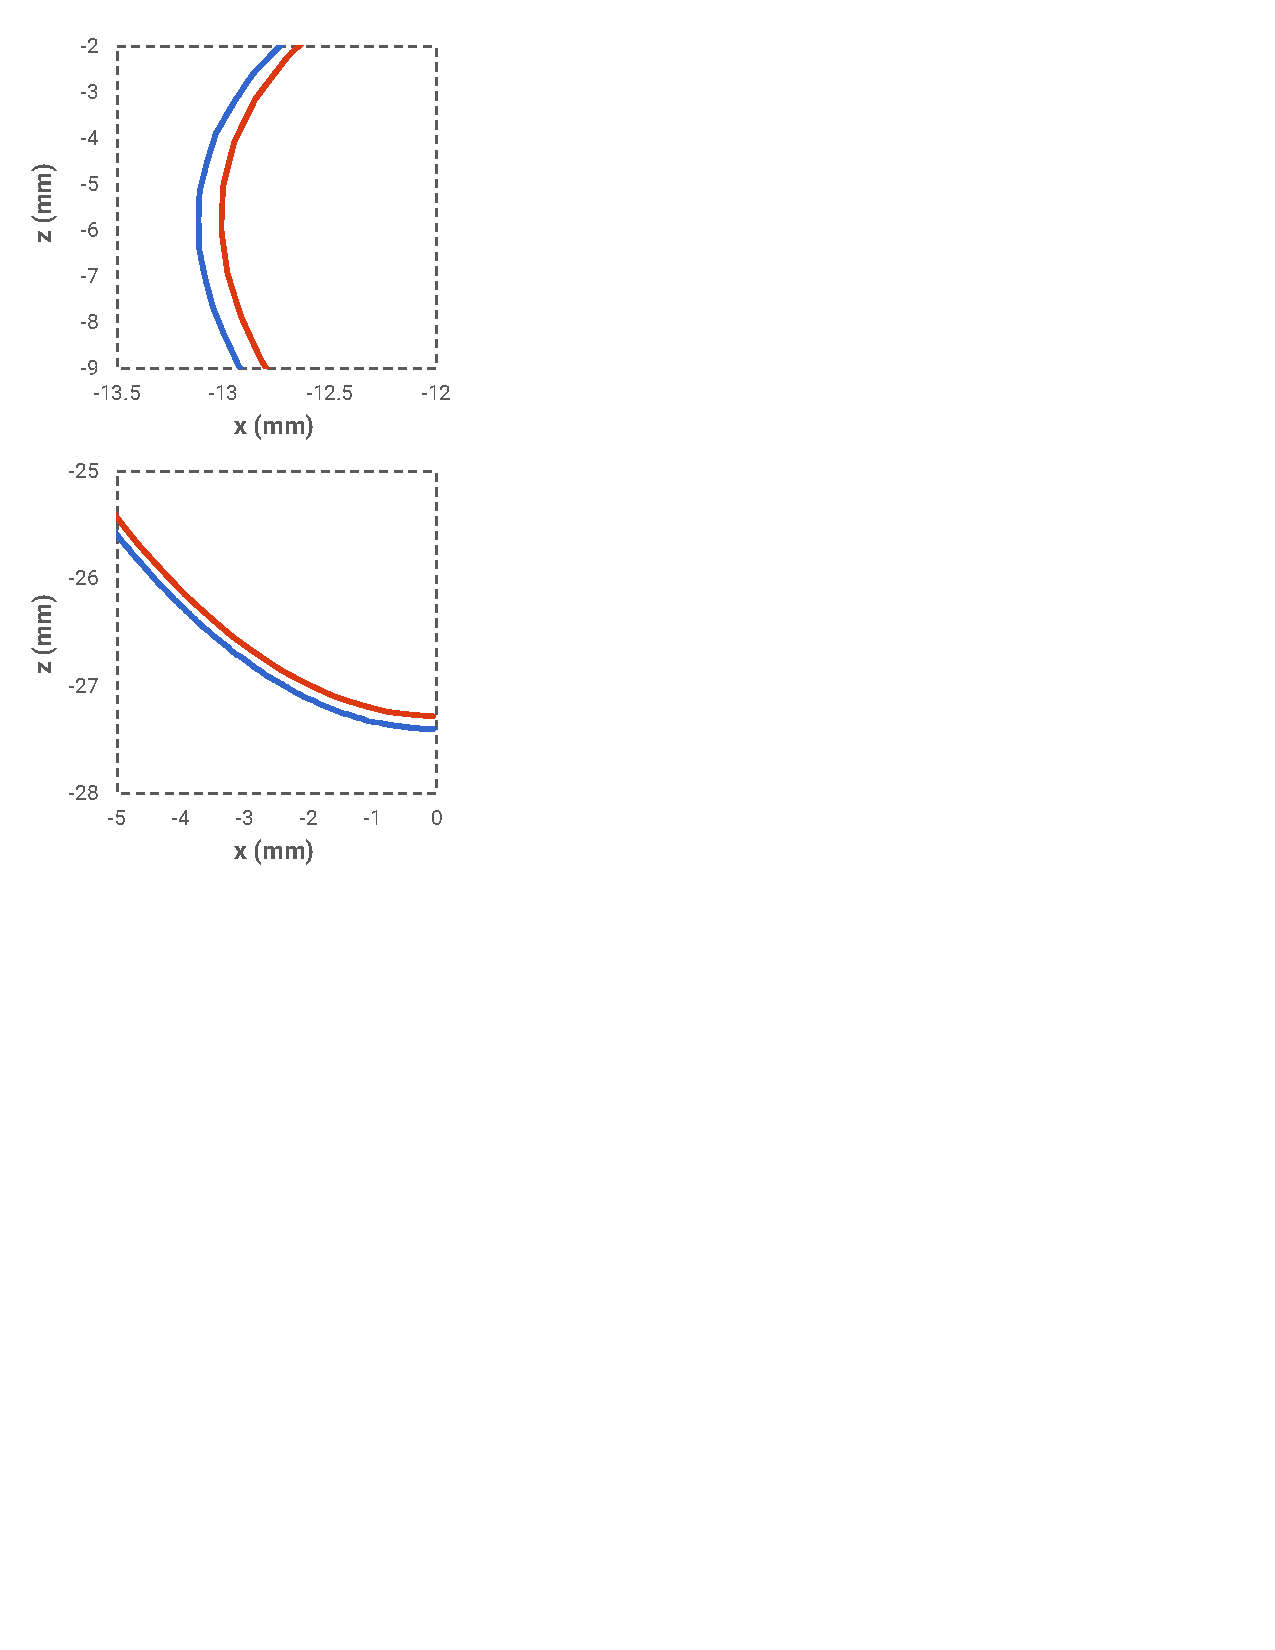
\includegraphics[scale=0.48]{media/5-verif/5-land2/land2-2.pdf}
\label{fig:land2-2}}	
\subfigure[]{%
		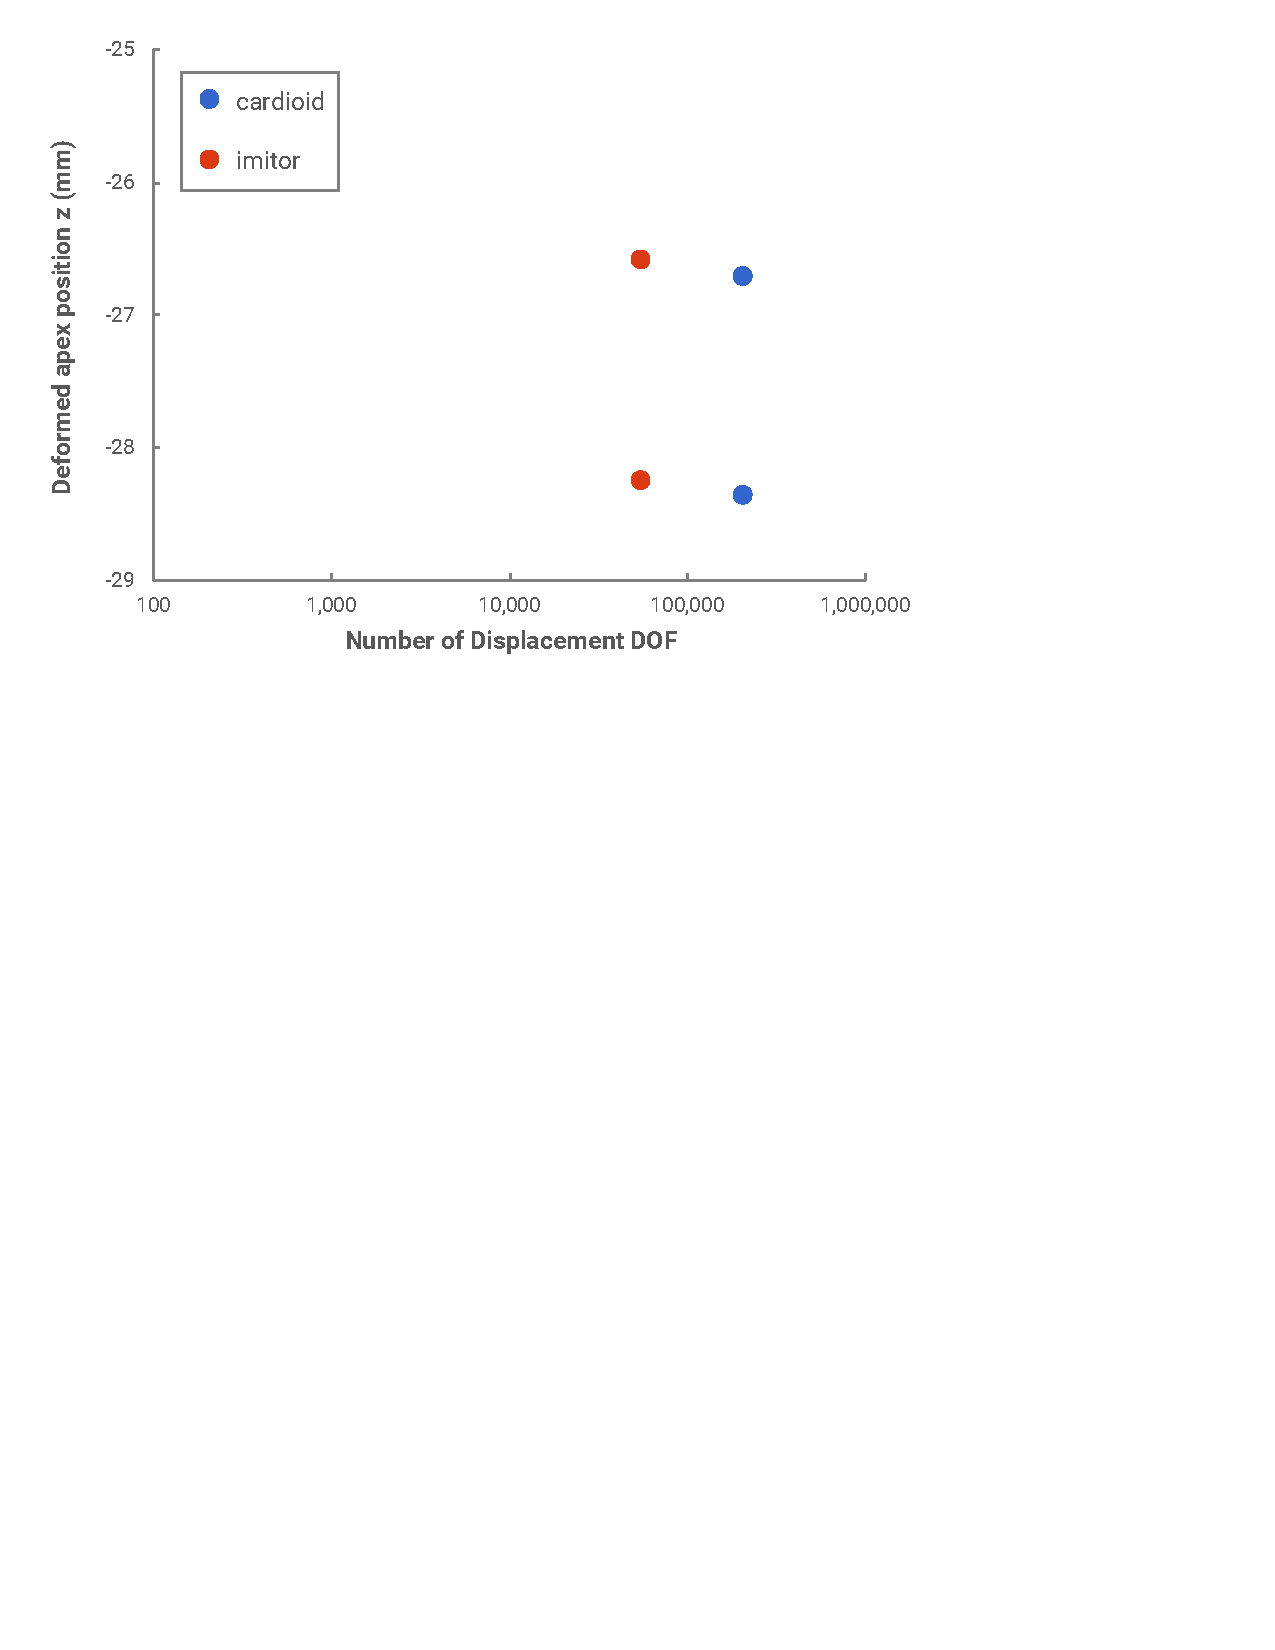
\includegraphics[scale=0.48]{media/5-verif/5-land2/land2-3.pdf}
\label{fig:land2-3}}			
%
\caption{Results for Land P2 verification problem: (a) Deformed position of middle of the ventricle wall, with (b) details at the inflection point (top right) and the apical region (bottom right). Panel (c) shows the deformed position of the apex at the endo- and epicardium for each of the simulation codes.}
\label{fig:land2}
\end{figure}

\begin{figure}[ht!]
\centering
\subfigure[]{%
		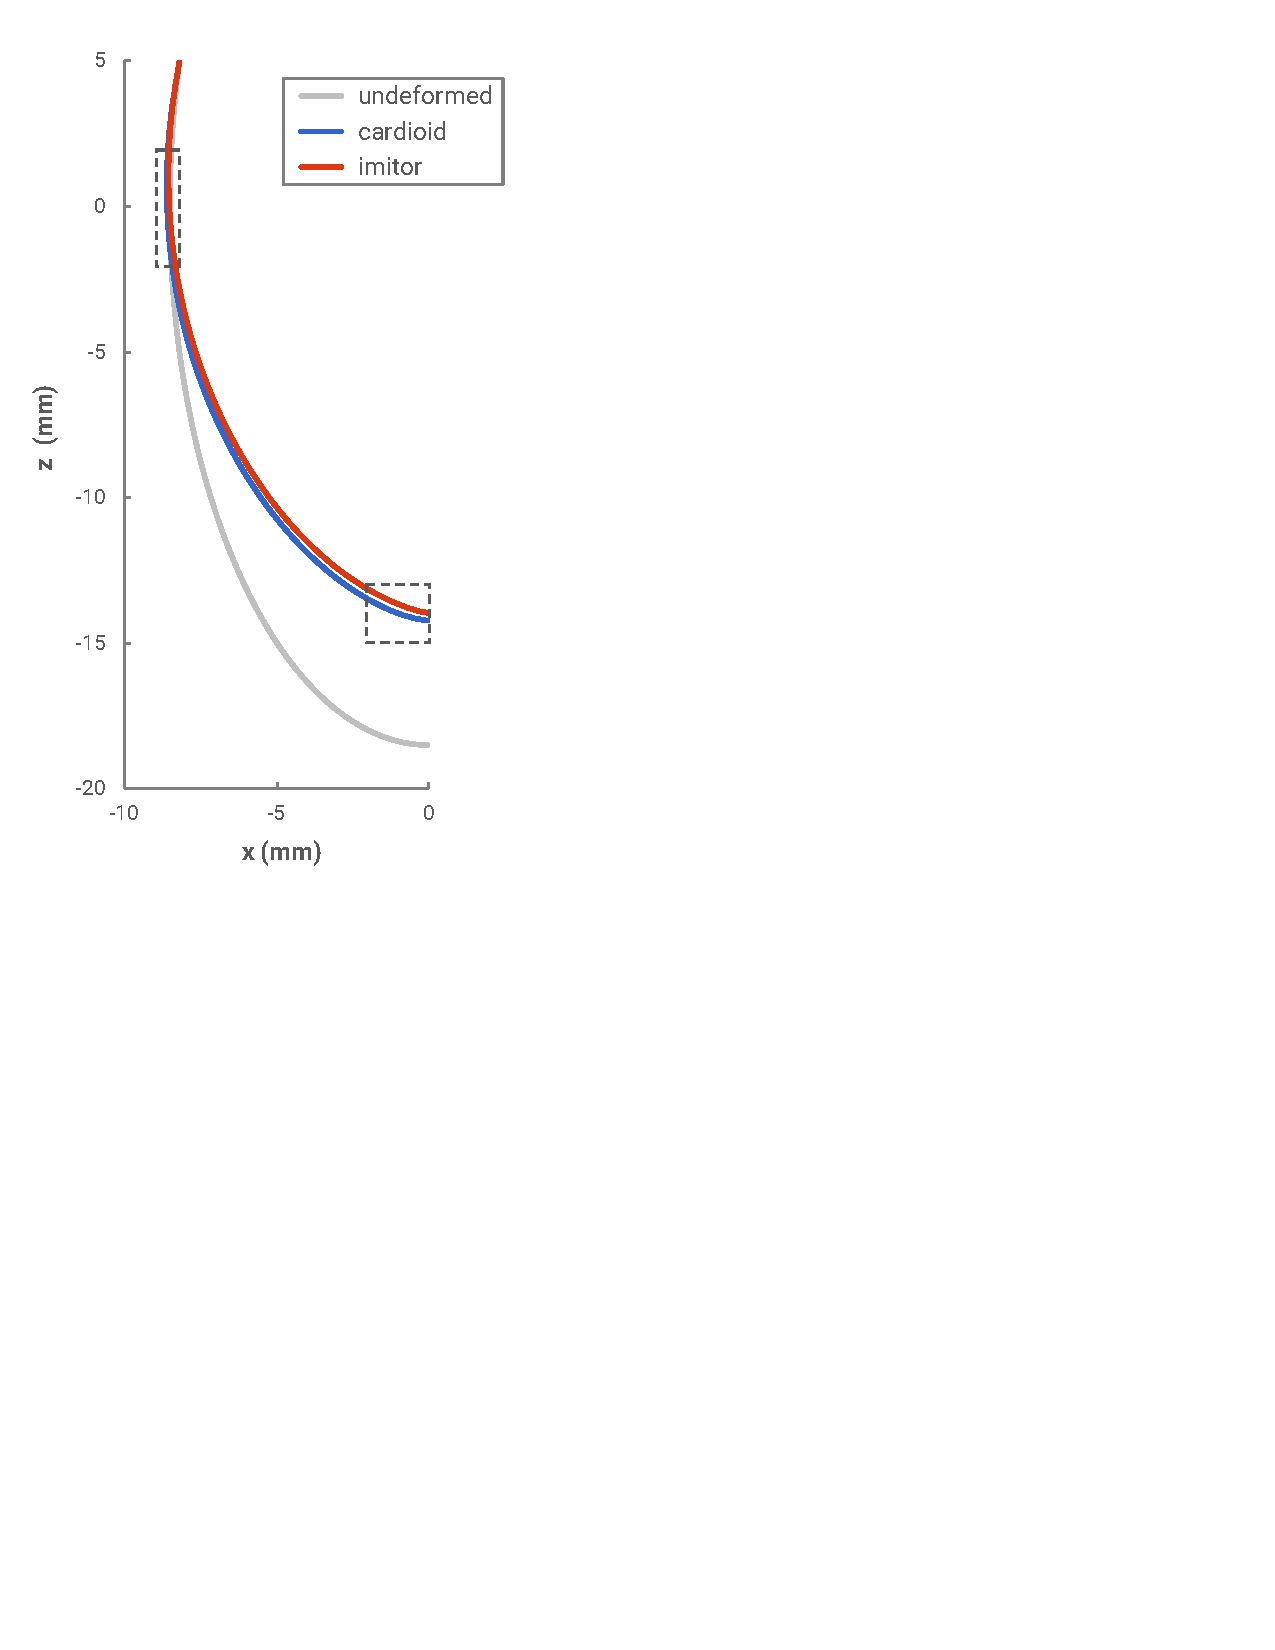
\includegraphics[scale=0.48]{media/5-verif/6-land3/land3-1.pdf}
\label{fig:land3-1}}		
\subfigure[]{%
		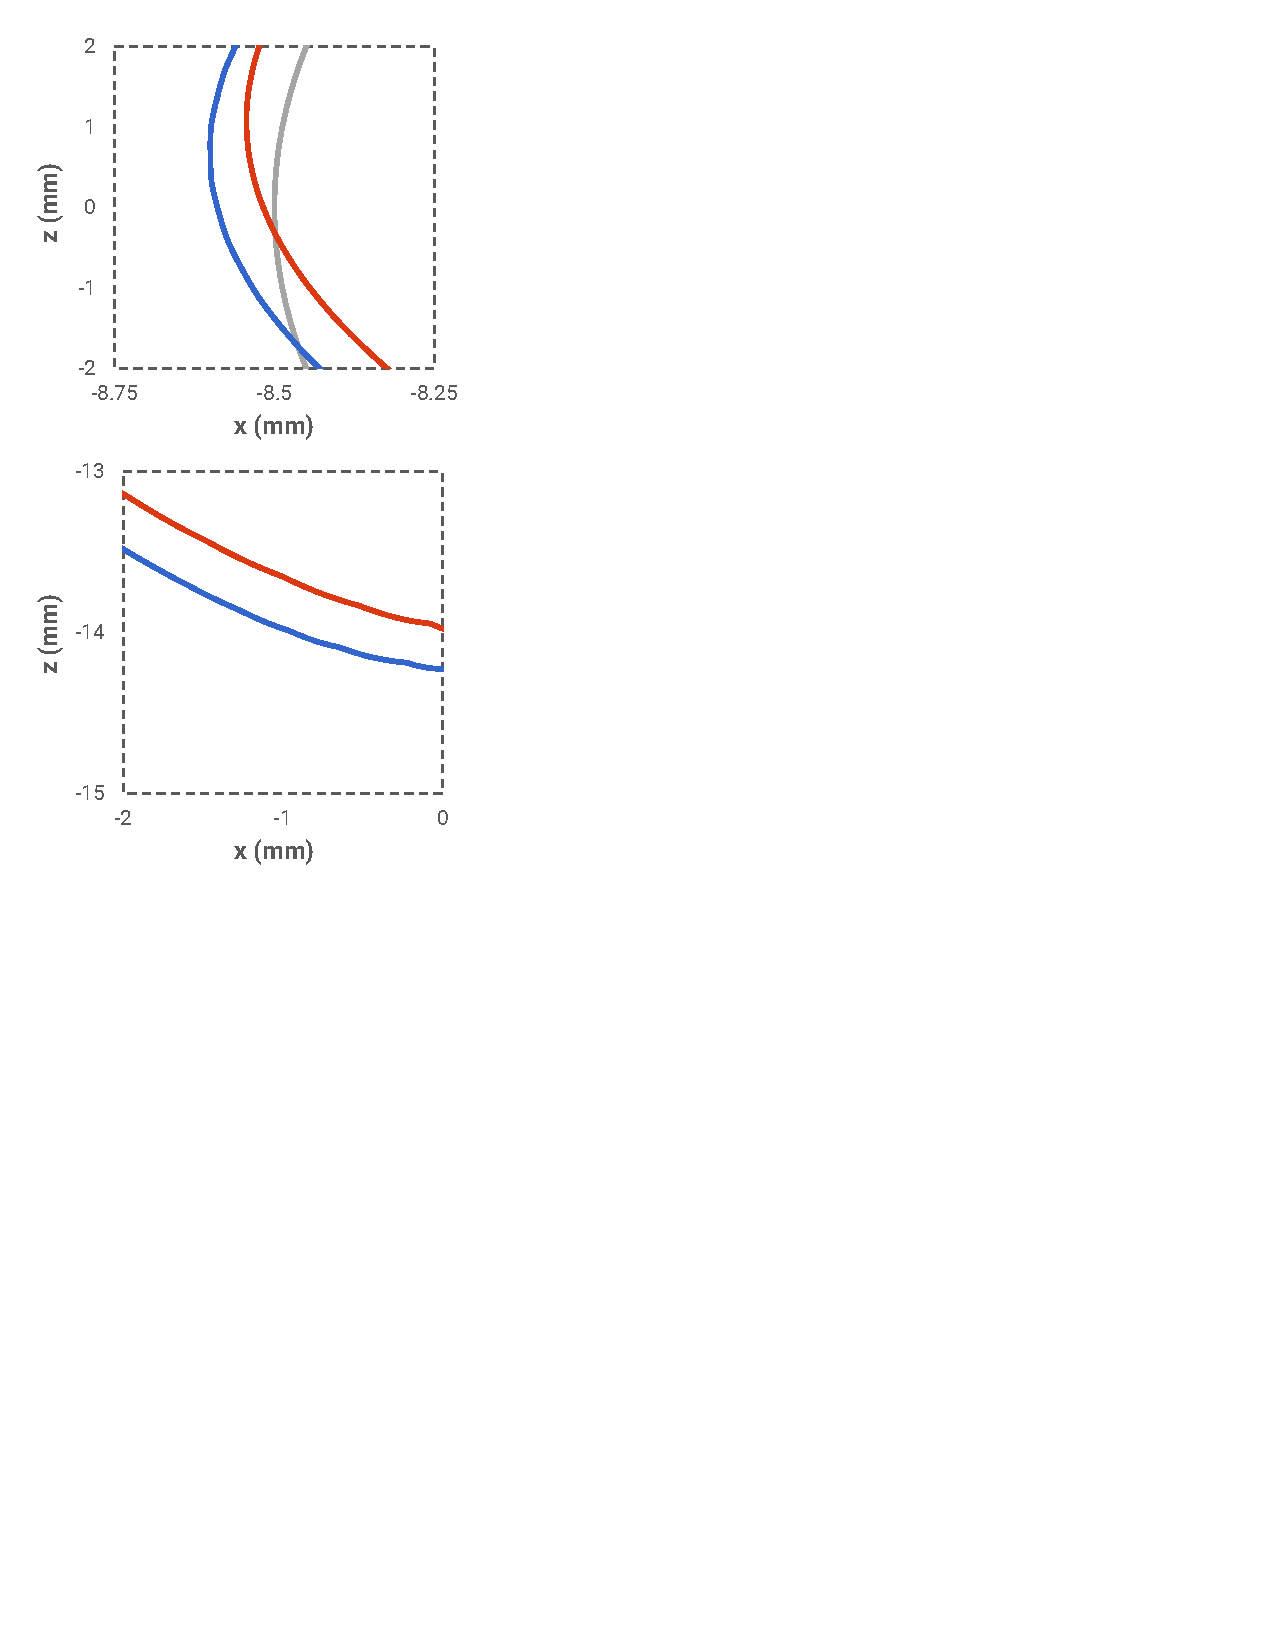
\includegraphics[scale=0.48]{media/5-verif/6-land3/land3-2.pdf}
\label{fig:land3-2}}	
%
\caption{Results for Land P3 verification problem: (a) Deformed position of middle of the ventricle wall, with (b) details at the inflection point (top right) and the apical region (bottom right).}
\label{fig:land3}
\end{figure}

\begin{figure}[ht!]
\centering
\subfigure[]{%
		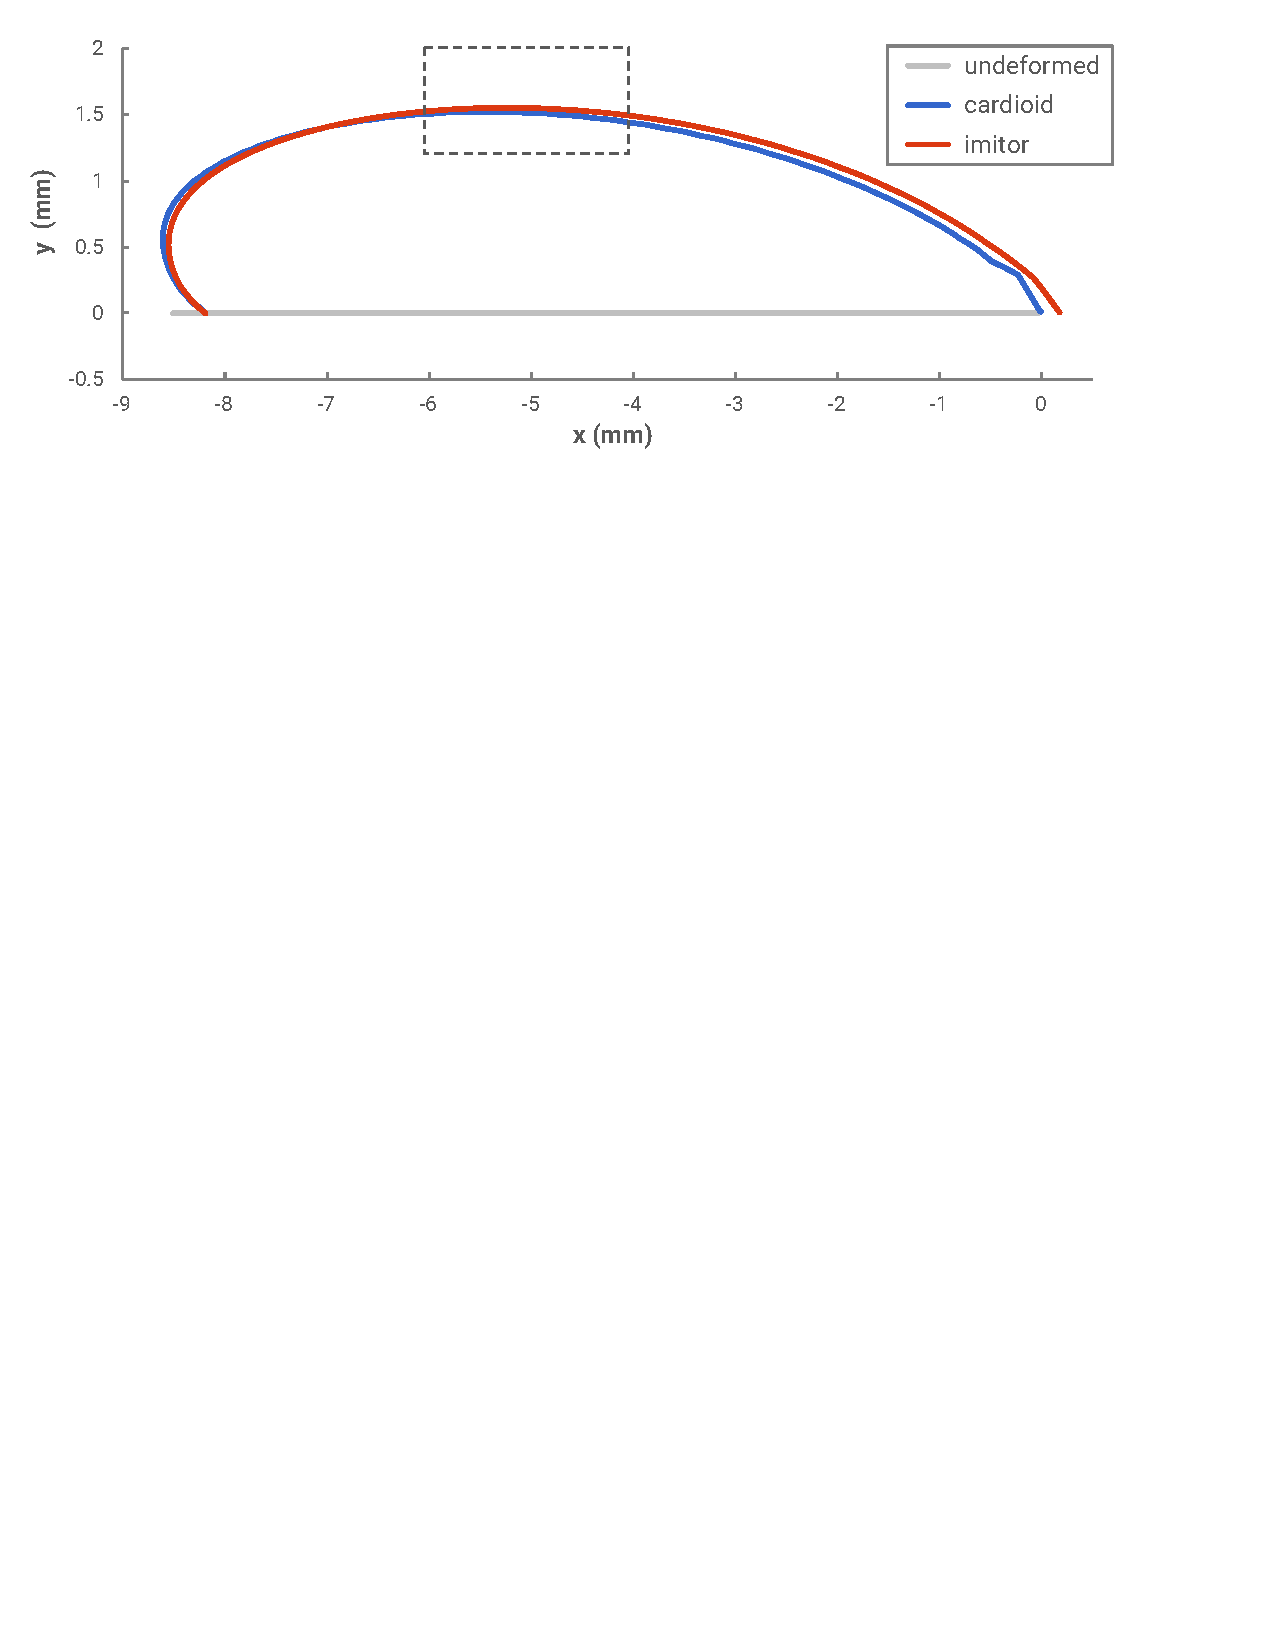
\includegraphics[scale=0.48]{media/5-verif/6-land3/land3-3.pdf}
\label{fig:land3.2-1}}		
\subfigure[]{%
		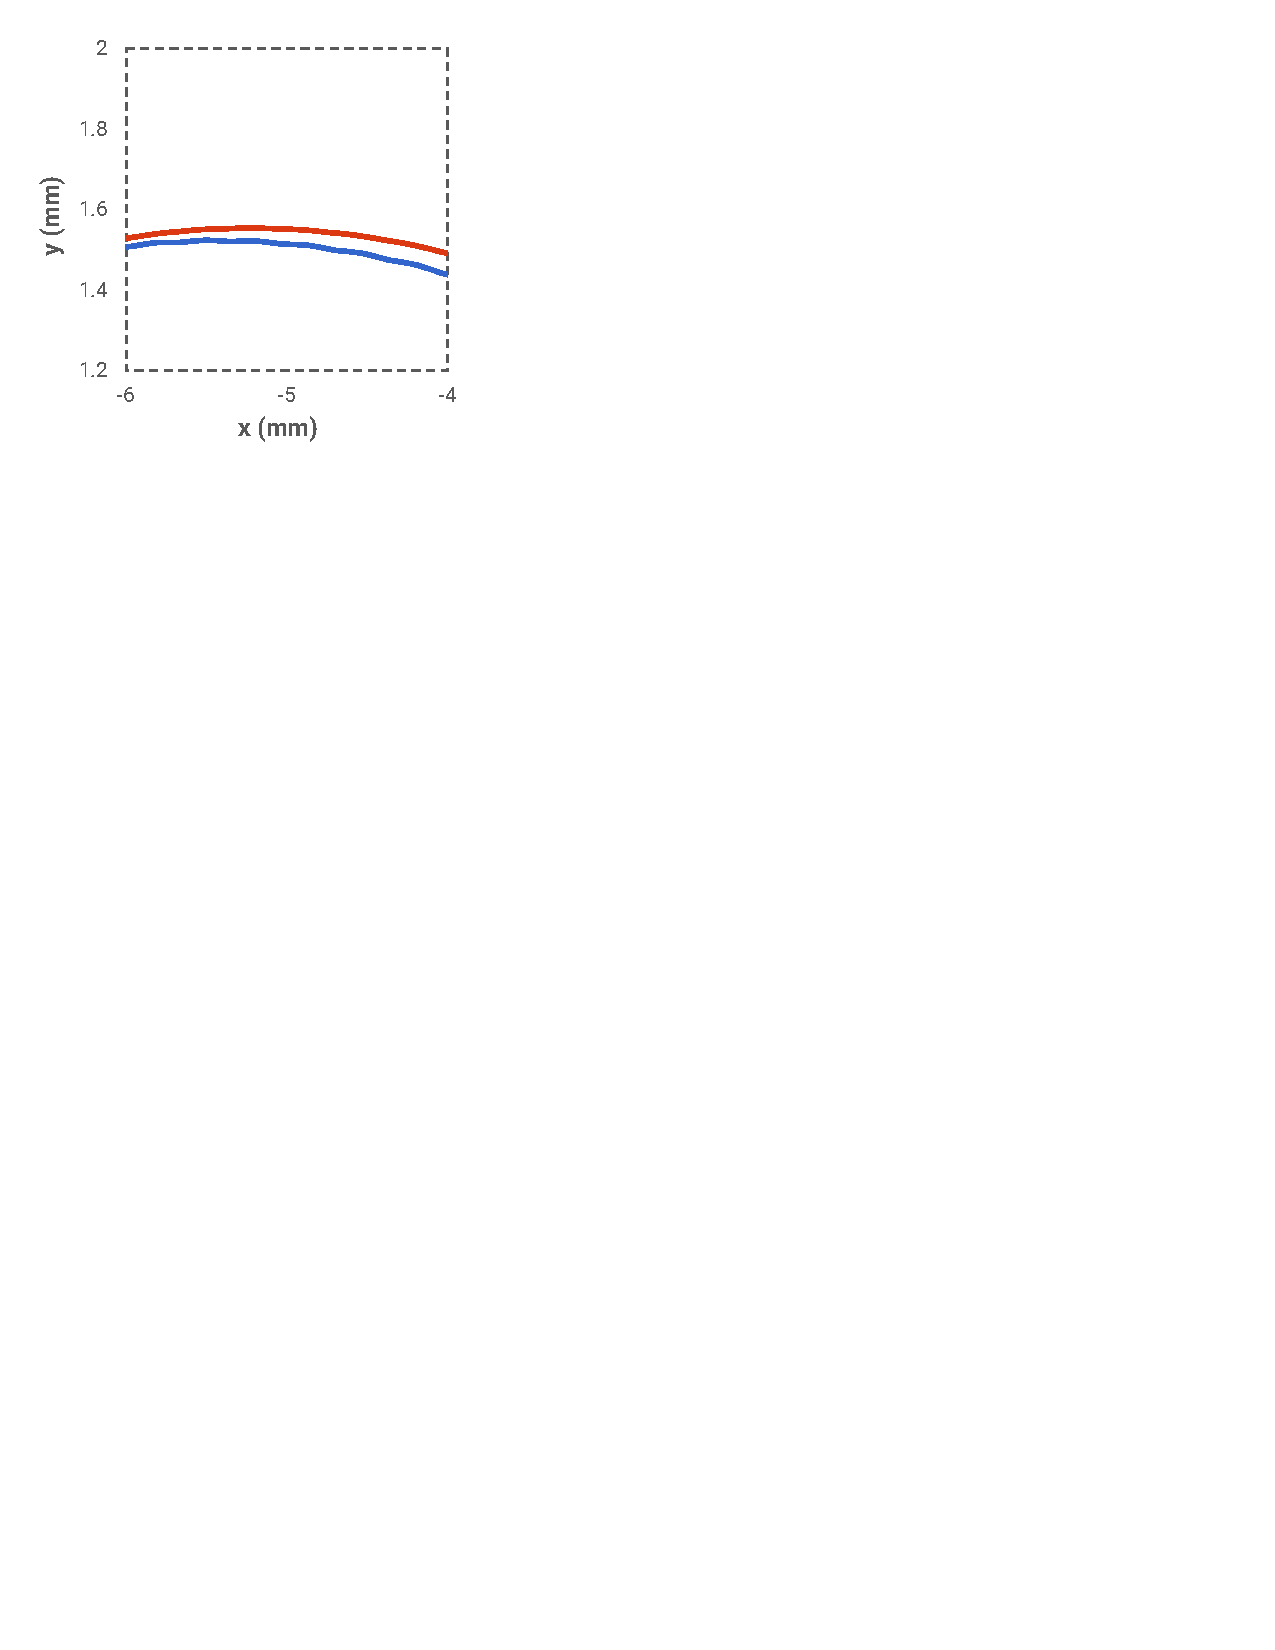
\includegraphics[scale=0.48]{media/5-verif/6-land3/land3-4.pdf}		
\label{fig:land3.2-2}}	
\subfigure[]{%
		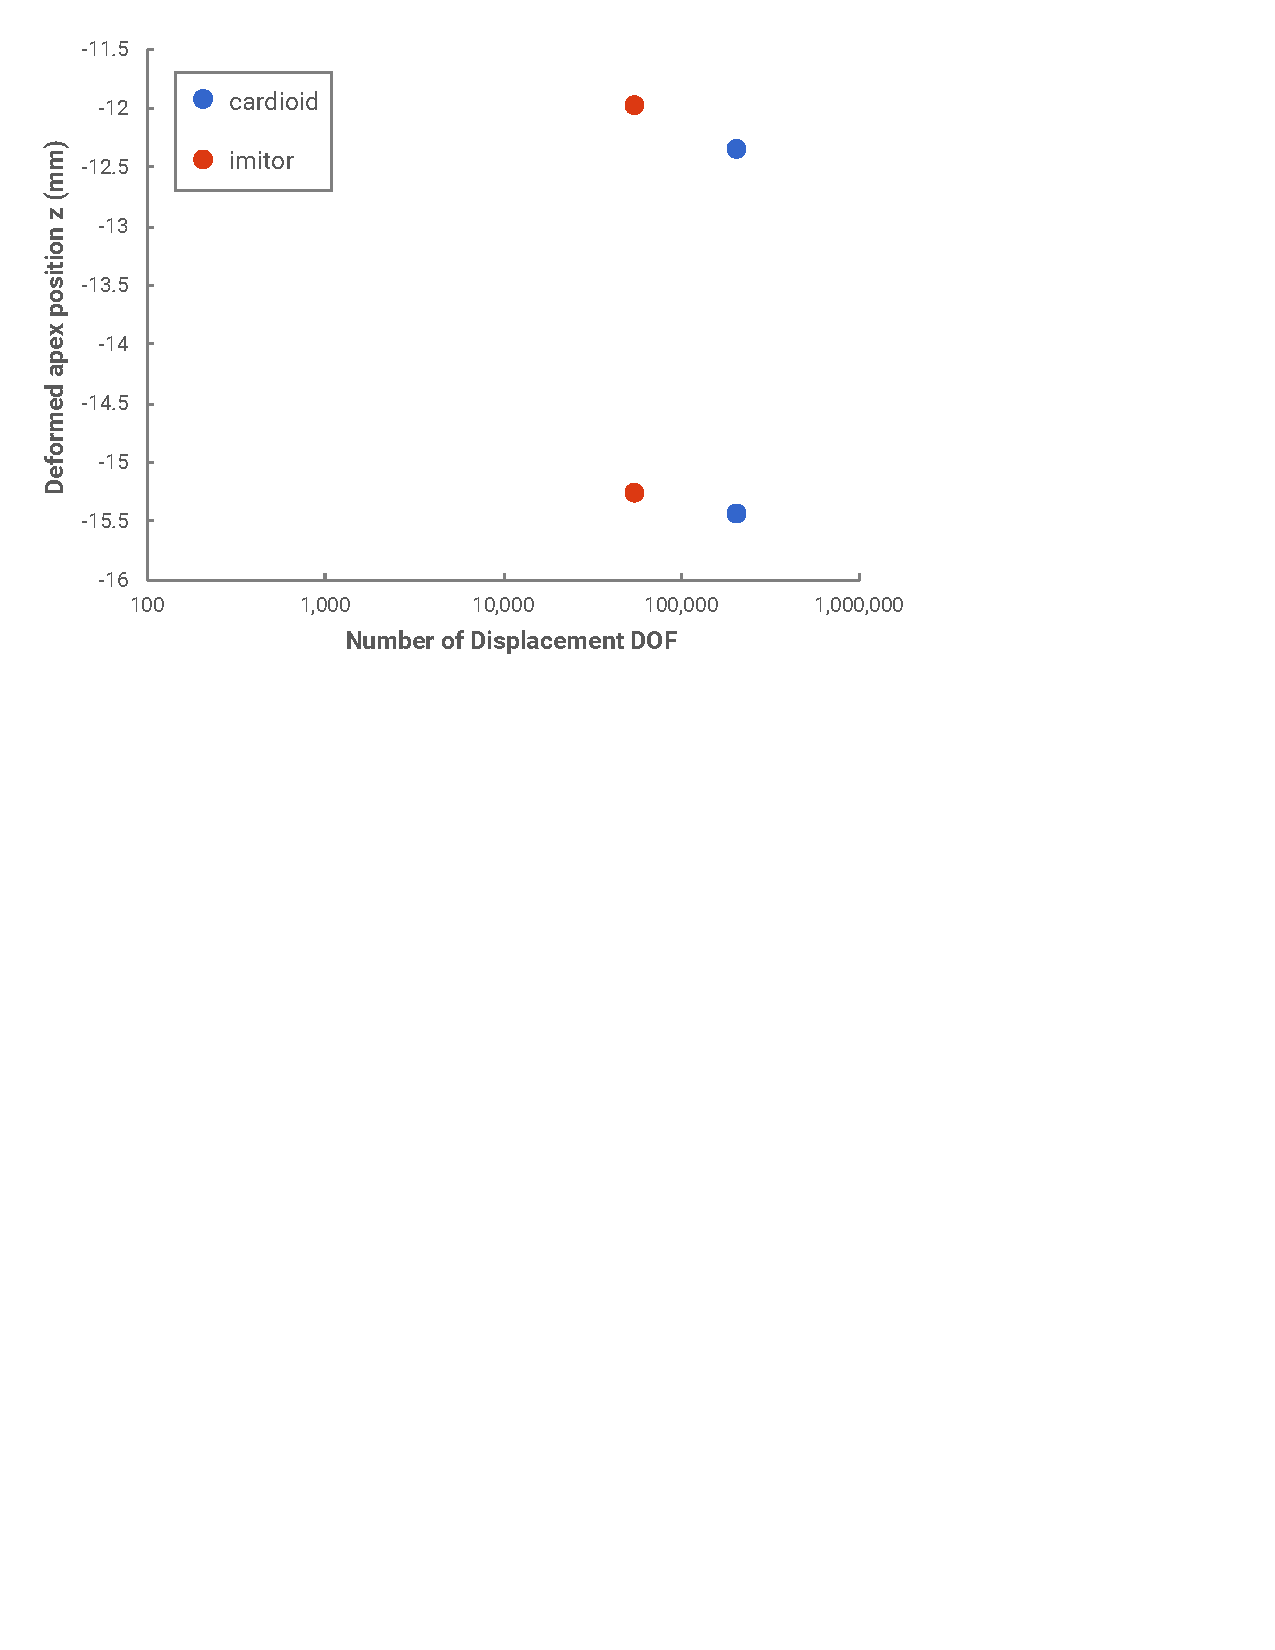
\includegraphics[scale=0.48]{media/5-verif/6-land3/land3-5.pdf}
\label{fig:land3.2-3}}			
	
%
\caption{Results for Land P3 verification problem: (a) The same deformed position of middle of the ventricle wall, shown in the $x-y$ plane, with (b) details at the inflection point. Panel (c) shows the deformed position of the apex at the endo- and epicardium for each of the simulation codes.}
\label{fig:land3.2}
\end{figure}
